\documentclass[12pt,a4paper]{report}

\usepackage{iftex}
\ifPDFTeX
  \usepackage[utf8]{inputenc}
  \usepackage[T1]{fontenc}
\else
  \usepackage{fontspec}
\fi

\usepackage[french]{babel}
\usepackage{geometry}
\geometry{margin=2.5cm}
\usepackage{graphicx}
\usepackage{xcolor}
\usepackage{booktabs}
\usepackage{longtable}
\usepackage{array}
\usepackage{tabularx}
\usepackage{enumitem}
\usepackage{caption}
\usepackage{float}
\usepackage{listings}
\usepackage{setspace}
\usepackage{fancyhdr}
\usepackage{titlesec}
\usepackage{amsmath}
\usepackage{amssymb}
\usepackage{microtype}
\usepackage{hyperref}

\hypersetup{
  colorlinks=true,
  linkcolor=blue!50!black,
  urlcolor=blue!60!black,
  citecolor=blue!50!black,
  pdftitle={Gestion des factures d'eau et d'electricite - Version finale},
  pdfauthor={Abdellah Bouarguan, Nafisa El Younoussi, Reda Zakaria, Nizar Ben Yacoub, Aymen Ouggourni}
}

\onehalfspacing
\setlength{\parskip}{0.2em}
\setlength{\headheight}{14pt}

\pagestyle{fancy}
\fancyhf{}
\fancyhead[L]{\small AquaVolt}
\fancyhead[R]{\small Version finale}
\fancyfoot[C]{\thepage}
\renewcommand{\headrulewidth}{0.4pt}

\titleformat{\chapter}[hang]
  {\bfseries\Large\color{blue!45!black}}
  {\thechapter}{1em}{}
\titlespacing*{\chapter}{0pt}{-10pt}{20pt}

\lstset{
  basicstyle=\ttfamily\small,
  breaklines=true,
  columns=fullflexible,
  frame=single,
  backgroundcolor=\color{gray!5},
  keywordstyle=\color{blue!70!black},
  commentstyle=\color{green!40!black},
  stringstyle=\color{red!60!black},
  showstringspaces=false,
  numbers=left,
  numberstyle=\tiny\color{gray},
  captionpos=b
}

\newcommand{\projectname}{AquaVolt}
\newcommand{\projectversion}{Version finale}
\newcommand{\projecttitle}{Gestion des factures d'eau et d'électricité}

% Marqueur visible pour les parties à compléter par les membres de l'équipe.
\newcommand{\todo}[1]{%
  \par\medskip\noindent
  \textit{\textcolor{gray!70}{À compléter : #1}}%
  \par\medskip
}

\begin{document}
\sloppy


\begin{titlepage}
    \centering
    \thispagestyle{empty}

    {\large Université Abdelmalek Essaâdi\par}
    \vspace{0.3cm}
    {\large École Nationale des Sciences Appliquées de Tétouan\par}
    \vspace{0.3cm}
    {\large Filière : Génie Informatique\par}

    \vspace{2.2cm}

    {\Huge\bfseries \projecttitle\par}
    \vspace{0.5cm}
    {\LARGE\bfseries \projectname\par}
    \vspace{0.3cm}
    {\large \projectversion\par}
    \vspace{0.3cm}
    {\large Mini-Projet 1\par}

    \vspace{2cm}

    {\large\bfseries Réalisé par :\par}
    \vspace{0.4cm}

    {\large
        Abdellah Bouarguan\\
        Nafisa El Younoussi\\
        Reda Zakaria\\
        Nizar Ben Yacoub\\
        Aymen Ouggourni\par
    }

    \vfill

    {\large Encadrant : Mohammed AL ACHHAB\par}
    \vspace{0.4cm}
    {\large Année universitaire : 2026--2027\par}
    {\large Date de remise : \today\par}

\end{titlepage}


\pagenumbering{roman}


\chapter*{Remerciements}
\addcontentsline{toc}{chapter}{Remerciements}

Nous tenons tout d'abord à exprimer notre profonde gratitude à notre encadrant, \textbf{Mohammed AL ACHHAB}, pour son accompagnement, ses conseils précieux et sa disponibilité tout au long de la réalisation de ce mini-projet.

Nous adressons également nos sincères remerciements à l'ensemble des membres de notre équipe pour leur engagement, leur collaboration et les efforts fournis durant les différentes étapes de conception, de développement et de validation de l'application AquaVolt.

Enfin, nous remercions l'École Nationale des Sciences Appliquées de Tétouan, ainsi que l'ensemble de son corps professoral, pour la formation dispensée et les connaissances acquises qui nous ont permis de mener à bien ce travail.

\chapter*{Résumé}
\addcontentsline{toc}{chapter}{Résumé}

\textbf{AquaVolt} est une application web dédiée à la gestion des consommations d'eau et d'électricité ainsi qu'au suivi de leurs factures. Elle a pour objectif de centraliser les différentes opérations liées à la gestion des clients, des contrats, des consommations et des paiements au sein d'une seule plateforme.

La version finale propose plusieurs fonctionnalités, notamment la gestion des clients et des quartiers, la saisie mensuelle des consommations avec téléversement des photographies des compteurs, la détection et le traitement des anomalies, ainsi que la génération automatique des factures. Elle intègre également la gestion des réclamations, l'enregistrement des paiements, l'importation et la vérification annuelles des consommations, les notifications internes et un tableau de bord destiné au suivi de l'activité du fournisseur.

Ce rapport présente les différentes étapes de réalisation du projet, depuis l'analyse des besoins et la conception de l'architecture jusqu'au développement des différents modules et à leur validation. Il expose également les mécanismes de sécurité adoptés, les tests réalisés et les perspectives d'amélioration de l'application.

\vspace{0.5cm}
\noindent\textbf{Mots-clés :} AquaVolt, PHP, gestion des consommations, facturation, eau, électricité, clients, contrats, anomalies, réclamations, paiements, notifications.

\chapter*{Abstract}
\addcontentsline{toc}{chapter}{Abstract}

\textbf{AquaVolt} is a web application for managing water and electricity consumption and related invoices. It is developed in PHP 8 with a MariaDB database and follows an MVC architecture that separates data access, business logic and the user interface.

The final version covers customer management, districts and contracts, monthly consumption entry with meter photographs, anomaly detection and processing, invoice generation and consultation, complaints, payments, annual import by an Agent, annual verification, internal notifications and the dashboard.

This report describes the project context, requirements analysis, architecture, data model, implemented modules, security mechanisms, tests and future improvements.

\vspace{0.5cm}
\noindent\textbf{Keywords:} PHP, MariaDB, MVC, consumption, billing, district, contract, complaint, payment, Agent, notifications, security.

\chapter*{Liste des abréviations}
\addcontentsline{toc}{chapter}{Liste des abréviations}

\begin{description}[leftmargin=3.2cm,style=nextline]
  \item[API] Interface de programmation applicative.
  \item[CRUD] Créer, lire, mettre à jour et supprimer.
  \item[CSRF] Cross-Site Request Forgery.
  \item[MVC] Modèle--Vue--Contrôleur.
  \item[PDO] PHP Data Objects.
  \item[SGBD] Système de gestion de base de données.
  \item[TVA] Taxe sur la valeur ajoutée.
  \item[UC] Cas d'utilisation.
  \item[XSS] Cross-Site Scripting.
\end{description}


\tableofcontents
\listoffigures
\listoftables

\clearpage
\pagenumbering{arabic}


\chapter*{Introduction générale}
\addcontentsline{toc}{chapter}{Introduction générale}

La gestion des consommations d'eau et d'électricité constitue une activité qui nécessite un suivi régulier des relevés des compteurs, une vérification des données collectées et un calcul précis des montants à facturer. La réalisation de ces opérations nécessite une organisation rigoureuse afin de garantir la fiabilité des informations et de limiter les erreurs de traitement.

Dans ce contexte, les applications web représentent une solution permettant de centraliser les différentes opérations au sein d'une plateforme unique. Elles facilitent la collecte des consommations, le suivi des factures, la gestion des réclamations et la consultation des informations par les différents acteurs concernés.

C'est dans cette perspective que s'inscrit le projet \textbf{AquaVolt}, une application web dédiée à la gestion des factures d'eau et d'électricité. Elle s'adresse à trois acteurs principaux : le client, qui peut transmettre ses relevés et consulter ses factures ; le fournisseur, qui assure la gestion des clients, des quartiers, des contrats, des anomalies, des réclamations et des paiements ; et l'agent, qui intervient notamment dans l'importation des consommations annuelles.

Développée en PHP 8 avec une base de données MariaDB et organisée selon l'architecture MVC, l'application regroupe les principales opérations liées au suivi des consommations et à la facturation. Elle intègre également des mécanismes de détection des anomalies, de vérification annuelle, de notification et de suivi de l'activité à travers un tableau de bord.

Le présent rapport décrit les différentes étapes de réalisation du projet. Il présente le contexte général, l'analyse des besoins, l'architecture technique, la conception de la base de données, les différents modules développés, les mécanismes de sécurité et les tests effectués. Enfin, il expose le bilan du travail réalisé ainsi que les limites et les perspectives d'évolution de l'application.

\section*{Organisation du rapport}

Le rapport est organisé en plusieurs chapitres complémentaires :

\begin{itemize}[leftmargin=*]
    \item le chapitre~\ref{chap:presentation} présente le projet, son contexte et son organisation ;
    \item le chapitre~\ref{chap:besoins} analyse les besoins fonctionnels et non fonctionnels ;
    \item le chapitre~\ref{chap:architecture} décrit l'architecture de l'application et les technologies utilisées ;
    \item le chapitre~\ref{chap:basededonnees} présente la conception et la structure de la base de données ;
    \item les chapitres suivants détaillent les différents modules fonctionnels de l'application ;
    \item le chapitre~\ref{chap:tests} présente les tests réalisés et leurs résultats ;
    \item le chapitre~\ref{chap:bilan} dresse le bilan du projet, ses limites et ses perspectives d'amélioration.
\end{itemize}

\chapter{Présentation du projet}
\label{chap:presentation}

\todo{présenter le contexte, la problématique, les objectifs, les acteurs et l'organisation du projet.}

\section{Contexte}
\section{Problématique}
\section{Objectifs}
\section{Acteurs et rôles}
\subsection{Client}
\subsection{Fournisseur}
\subsection{Agent}
\section{Périmètre de la version finale}
\section{Méthodologie de travail}
\section{Répartition des tâches}
\section{Planning et réunions}

\chapter{Analyse des besoins}
\label{chap:besoins}

\todo{présenter les besoins fonctionnels, non fonctionnels, les règles métier et les cas d'utilisation.}

\section{Besoins fonctionnels}
\subsection{Client}
\subsection{Fournisseur}
\subsection{Agent}
\section{Besoins non fonctionnels}
\section{Règles métier}
\section{Cas d'utilisation}
\section{Scénarios principaux}
\section{Contraintes et hypothèses}

\chapter{Architecture et technologies}
\label{chap:architecture}

\todo{décrire l'architecture MVC, le routeur, l'organisation des fichiers et les technologies.}

\section{Architecture MVC}
\subsection{Modèle}
\subsection{Vue}
\subsection{Contrôleur}
\section{Routeur et cycle d'une requête}
\section{Organisation des fichiers}
\section{Technologies utilisées}
\section{Environnement de développement}
\section{Choix de conception}


\chapter{Base de données}
\label{chap:basededonnees}

\section{Modèle conceptuel}

La base de données d'AquaVolt est conçue pour centraliser les informations nécessaires à la gestion des clients, des contrats, des consommations d'eau et d'électricité, des factures et des opérations associées.

Elle repose sur plusieurs entités liées entre elles par des relations permettant de garantir la cohérence des informations.

Les principales entités du système sont :

\begin{itemize}[leftmargin=*]
    \item \textbf{Fournisseur :} représente l'organisme responsable de la gestion des clients et des tarifs.
    \item \textbf{Agent :} représente l'utilisateur chargé de l'importation des consommations annuelles.
    \item \textbf{Client :} représente l'abonné utilisant les services d'eau et d'électricité.
    \item \textbf{Quartier :} représente une zone géographique caractérisée par un type d'activité.
    \item \textbf{Contrat :} représente l'engagement entre un client et le service associé à un quartier.
    \item \textbf{Tarif :} définit les prix unitaires applicables selon le type de consommation et les tranches.
    \item \textbf{Consommation :} enregistre les index mensuels d'eau et d'électricité.
    \item \textbf{Photo\_capteur :} conserve les chemins des photographies associées aux relevés.
    \item \textbf{Anomalie :} enregistre les incohérences détectées dans les relevés.
    \item \textbf{Facture :} conserve les informations relatives à la facturation et au paiement.
    \item \textbf{Réclamation :} enregistre les demandes et signalements déposés par les clients.
    \item \textbf{Notification :} conserve les messages destinés aux différents utilisateurs.
    \item \textbf{Conso\_annuelle :} conserve les consommations annuelles importées par l'Agent.
\end{itemize}

Les relations entre ces entités permettent de représenter les différents processus métier de l'application.

\section{Modèle logique}

Le modèle logique est implémenté dans une base de données relationnelle nommée \texttt{miniproject\_version\_alpha}. Il utilise le moteur de stockage InnoDB et l'encodage UTF-8 avec le jeu de caractères \texttt{utf8mb4}.

Chaque table possède une clé primaire permettant d'identifier ses enregistrements. Les relations entre les tables sont établies à l'aide de clés étrangères.

Les principales associations sont les suivantes :

\begin{itemize}[leftmargin=*]
    \item Un fournisseur possède plusieurs clients et plusieurs tarifs.
    \item Un client peut posséder plusieurs contrats et plusieurs consommations.
    \item Un quartier peut être associé à plusieurs contrats.
    \item Un contrat possède plusieurs relevés mensuels.
    \item Une consommation peut être associée à des photographies et à des anomalies.
    \item Une consommation peut donner lieu à une facture unique.
    \item Un client peut déposer plusieurs réclamations.
    \item Un agent peut importer plusieurs relevés annuels.
    \item Un utilisateur peut recevoir plusieurs notifications.
\end{itemize}

\section{Description des tables}

La base de données comprend treize tables principales. Les sections suivantes présentent leur rôle et leurs principaux attributs.

\subsection{fournisseur}

La table \texttt{fournisseur} contient les informations relatives au fournisseur responsable de la gestion de la plateforme.

\begin{itemize}[leftmargin=*]
    \item \texttt{id\_fournisseur} : identifiant unique du fournisseur.
    \item \texttt{nom} : nom du fournisseur.
    \item \texttt{email} : adresse électronique, unique.
    \item \texttt{mot\_de\_passe} : mot de passe enregistré.
    \item \texttt{seuil\_eau} : seuil maximal défini pour la consommation d'eau.
    \item \texttt{seuil\_elec} : seuil maximal défini pour la consommation d'électricité.
    \item \texttt{date\_creation} : date de création de l'enregistrement.
\end{itemize}

\subsection{client}

La table \texttt{client} regroupe les informations personnelles et les informations d'accès des clients.

\begin{itemize}[leftmargin=*]
    \item \texttt{id\_client} : identifiant unique du client.
    \item \texttt{id\_fournisseur} : référence au fournisseur associé.
    \item \texttt{cin} : numéro de la carte d'identité nationale.
    \item \texttt{nom}, \texttt{prenom} : identité du client.
    \item \texttt{adresse} : adresse du client.
    \item \texttt{email} : adresse électronique unique.
    \item \texttt{mot\_de\_passe} : mot de passe enregistré.
    \item \texttt{telephone} : numéro de téléphone facultatif.
    \item \texttt{date\_creation} : date de création du compte.
\end{itemize}

\subsection{quartier}

La table \texttt{quartier} représente les quartiers pris en charge par l'application.

\begin{itemize}[leftmargin=*]
    \item \texttt{id\_quartier} : identifiant unique du quartier.
    \item \texttt{nom} : nom du quartier.
    \item \texttt{type\_activite} : type d'activité (\texttt{RESIDENTIEL}, \texttt{COMMERCIAL} ou \texttt{INDUSTRIEL}).
    \item \texttt{date\_creation} : date de création.
\end{itemize}

L'association entre le nom du quartier et son type d'activité doit être unique.

\subsection{contrat}

La table \texttt{contrat} permet de représenter les contrats associés aux clients et aux quartiers.

\begin{itemize}[leftmargin=*]
    \item \texttt{id\_contrat} : identifiant unique du contrat.
    \item \texttt{id\_client} : référence au client concerné.
    \item \texttt{id\_quartier} : référence au quartier associé.
    \item \texttt{numero\_contrat} : numéro unique du contrat.
    \item \texttt{date\_debut} : date de début du contrat.
    \item \texttt{date\_fin} : date de fin éventuelle.
    \item \texttt{statut} : état du contrat (\texttt{ACTIF} ou \texttt{RESILIE}).
    \item \texttt{date\_creation} : date de création de l'enregistrement.
\end{itemize}

\subsection{tarif}

La table \texttt{tarif} contient les tarifs appliqués par le fournisseur pour les consommations d'eau et d'électricité.

\begin{itemize}[leftmargin=*]
    \item \texttt{id\_tarif} : identifiant unique du tarif.
    \item \texttt{id\_fournisseur} : référence au fournisseur.
    \item \texttt{type} : type de consommation (\texttt{EAU} ou \texttt{ELEC}).
    \item \texttt{borne\_min} : limite inférieure de la tranche.
    \item \texttt{borne\_max} : limite supérieure de la tranche, éventuellement nulle pour la dernière tranche.
    \item \texttt{prix\_unitaire} : prix appliqué à l'unité consommée.
\end{itemize}

Les tranches sont représentées par des intervalles de la forme
\texttt{[borne\_min, borne\_max[}. Une borne maximale nulle indique une dernière tranche sans limite supérieure.

\subsection{consommation}

La table \texttt{consommation} enregistre les relevés mensuels des compteurs d'eau et d'électricité.

\begin{itemize}[leftmargin=*]
    \item \texttt{id\_conso} : identifiant unique du relevé.
    \item \texttt{id\_client} : référence au client.
    \item \texttt{id\_contrat} : référence au contrat concerné.
    \item \texttt{periode\_mois} : mois du relevé.
    \item \texttt{periode\_annee} : année du relevé.
    \item \texttt{index\_eau} : index du compteur d'eau.
    \item \texttt{index\_elec} : index du compteur d'électricité.
    \item \texttt{date\_saisie} : date d'enregistrement du relevé.
    \item \texttt{statut} : état du relevé.
\end{itemize}

Un contrat ne peut posséder qu'un seul relevé pour une même période mensuelle.

\subsection{photo\_capteur}

La table \texttt{photo\_capteur} conserve les références des photographies associées aux relevés des compteurs.

\begin{itemize}[leftmargin=*]
    \item \texttt{id\_photo} : identifiant unique de la photographie.
    \item \texttt{id\_conso} : référence à la consommation concernée.
    \item \texttt{type} : type de compteur (\texttt{EAU} ou \texttt{ELEC}).
    \item \texttt{chemin} : chemin du fichier photographique.
    \item \texttt{date\_televersement} : date du téléversement.
\end{itemize}

La contrainte d'unicité sur \texttt{id\_conso} et \texttt{type} limite à une seule photographie par type de compteur pour chaque consommation.

\subsection{anomalie}

La table \texttt{anomalie} permet d'enregistrer les incohérences détectées lors de la vérification des relevés.

\begin{itemize}[leftmargin=*]
    \item \texttt{id\_anomalie} : identifiant unique de l'anomalie.
    \item \texttt{id\_conso} : référence au relevé concerné.
    \item \texttt{id\_fournisseur} : référence au fournisseur chargé du traitement.
    \item \texttt{type\_anomalie} : type d'anomalie (\texttt{INDEX\_INFERIEUR} ou \texttt{SEUIL\_DEPASSE}).
    \item \texttt{champ} : compteur concerné (\texttt{EAU} ou \texttt{ELEC}).
    \item \texttt{valeur\_saisie} : valeur initialement saisie.
    \item \texttt{valeur\_reference} : valeur utilisée comme référence.
    \item \texttt{statut} : état de traitement de l'anomalie.
    \item \texttt{valeur\_corrigee} : valeur corrigée éventuelle.
    \item \texttt{date\_detection} : date de détection.
    \item \texttt{date\_resolution} : date de résolution éventuelle.
\end{itemize}

\subsection{facture}

La table \texttt{facture} contient les informations relatives aux factures générées à partir des consommations.

\begin{itemize}[leftmargin=*]
    \item \texttt{id\_facture} : identifiant unique de la facture.
    \item \texttt{numero} : numéro unique de la facture.
    \item \texttt{id\_client} : référence au client.
    \item \texttt{id\_conso} : référence à la consommation facturée.
    \item \texttt{date\_facture} : date d'émission.
    \item \texttt{periode\_mois} et \texttt{periode\_annee} : période facturée.
    \item \texttt{conso\_eau} et \texttt{conso\_elec} : consommations facturées.
    \item \texttt{montant\_ht} : montant hors taxes.
    \item \texttt{taux\_tva} : taux de TVA, fixé par défaut à 18\,\%.
    \item \texttt{montant\_tva} : montant de la TVA.
    \item \texttt{montant\_ttc} : montant toutes taxes comprises.
    \item \texttt{etat} : état de la facture (\texttt{IMPAYEE} ou \texttt{PAYEE}).
    \item \texttt{date\_paiement} : date du paiement éventuel.
    \item \texttt{mode\_paiement} : mode de paiement.
    \item \texttt{reference\_paiement} : référence du paiement.
\end{itemize}

La table permet ainsi de conserver les informations de facturation et de paiement sans utiliser une table de paiement distincte.

\subsection{notification}

La table \texttt{notification} conserve les notifications internes destinées aux différents utilisateurs de l'application.

\begin{itemize}[leftmargin=*]
    \item \texttt{id\_notification} : identifiant unique de la notification.
    \item \texttt{destinataire\_role} : rôle du destinataire (\texttt{client}, \texttt{fournisseur} ou \texttt{agent}).
    \item \texttt{id\_destinataire} : identifiant du destinataire.
    \item \texttt{type} : catégorie de notification.
    \item \texttt{titre} : titre du message.
    \item \texttt{message} : contenu de la notification.
    \item \texttt{lien} : lien facultatif vers une fonctionnalité.
    \item \texttt{lu} : indicateur de lecture.
    \item \texttt{date\_creation} : date de création.
    \item \texttt{date\_lecture} : date de lecture éventuelle.
\end{itemize}

Le destinataire est identifié par la combinaison de son rôle et de son identifiant. Cette conception permet de gérer plusieurs catégories d'utilisateurs dans une même table.

\subsection{agent}

La table \texttt{agent} contient les informations relatives aux agents chargés notamment de l'importation annuelle.

\begin{itemize}[leftmargin=*]
    \item \texttt{id\_agent} : identifiant unique de l'agent.
    \item \texttt{nom} et \texttt{prenom} : identité de l'agent.
    \item \texttt{email} : adresse électronique unique.
    \item \texttt{mot\_de\_passe} : mot de passe enregistré.
    \item \texttt{telephone} : numéro de téléphone facultatif.
    \item \texttt{date\_creation} : date de création du compte.
\end{itemize}

\subsection{conso\_annuelle}

La table \texttt{conso\_annuelle} conserve les relevés annuels issus de la tournée de l'Agent.

\begin{itemize}[leftmargin=*]
    \item \texttt{id\_conso\_annuelle} : identifiant unique du relevé annuel.
    \item \texttt{id\_client} : référence au client concerné.
    \item \texttt{id\_agent} : référence à l'agent ayant effectué l'importation.
    \item \texttt{conso\_eau} : consommation annuelle d'eau.
    \item \texttt{conso\_elec} : consommation annuelle d'électricité.
    \item \texttt{annee} : année concernée.
    \item \texttt{date\_saisie} : date d'enregistrement.
    \item \texttt{statut\_verification} : état de vérification.
    \item \texttt{date\_verification} : date de vérification éventuelle.
\end{itemize}

La combinaison du client et de l'année est unique, ce qui empêche l'enregistrement de plusieurs relevés annuels pour un même client durant la même année.

\subsection{reclamation}

La table \texttt{reclamation} permet de gérer les réclamations déposées par les clients.

\begin{itemize}[leftmargin=*]
    \item \texttt{id\_reclamation} : identifiant unique de la réclamation.
    \item \texttt{numero} : numéro unique de la réclamation.
    \item \texttt{id\_client} : référence au client concerné.
    \item \texttt{id\_facture} : référence facultative à une facture.
    \item \texttt{type} : type de réclamation.
    \item \texttt{description} : description du problème signalé.
    \item \texttt{piece\_jointe} : chemin d'une pièce jointe éventuelle.
    \item \texttt{statut} : état de traitement.
    \item \texttt{reponse} : réponse éventuelle du fournisseur.
    \item \texttt{date\_creation} : date de dépôt.
    \item \texttt{date\_resolution} : date de résolution éventuelle.
\end{itemize}

\section{Relations et cardinalités}

Les relations entre les tables sont définies à l'aide de clés étrangères. Les principales cardinalités du modèle sont présentées dans le tableau suivant.

\begin{table}[H]
    \centering
    \caption{Principales relations entre les entités}
    \begin{tabularx}{\textwidth}{|l|l|X|}
        \hline
        \textbf{Entités liées} & \textbf{Cardinalité} & \textbf{Signification} \\
        \hline
        Fournisseur -- Client & 1,N & Un fournisseur peut gérer plusieurs clients. \\
        \hline
        Fournisseur -- Tarif & 1,N & Un fournisseur peut définir plusieurs tarifs. \\
        \hline
        Client -- Contrat & 1,N & Un client peut posséder plusieurs contrats. \\
        \hline
        Quartier -- Contrat & 1,N & Un quartier peut être associé à plusieurs contrats. \\
        \hline
        Client -- Consommation & 1,N & Un client peut posséder plusieurs relevés. \\
        \hline
        Contrat -- Consommation & 1,N & Un contrat peut posséder plusieurs relevés mensuels. \\
        \hline
        Consommation -- Photo\_capteur & 1,N & Un relevé peut être associé à plusieurs photographies. \\
        \hline
        Consommation -- Anomalie & 1,N & Un relevé peut présenter plusieurs anomalies. \\
        \hline
        Consommation -- Facture & 1,1 & Une consommation peut être associée à une seule facture au maximum. \\
        \hline
        Client -- Facture & 1,N & Un client peut recevoir plusieurs factures. \\
        \hline
        Client -- Réclamation & 1,N & Un client peut déposer plusieurs réclamations. \\
        \hline
        Agent -- Conso\_annuelle & 1,N & Un agent peut être associé à plusieurs relevés annuels. \\
        \hline
        Client -- Conso\_annuelle & 1,N & Un client peut avoir plusieurs relevés annuels, un par année. \\
        \hline
    \end{tabularx}
\end{table}

La relation entre une facture et une réclamation est facultative du côté de la réclamation : une réclamation peut concerner une facture précise ou être indépendante d'une facture.

La table \texttt{notification} constitue un cas particulier. Elle identifie son destinataire à l'aide de deux attributs, \texttt{destinataire\_role} et \texttt{id\_destinataire}, sans clé étrangère directe vers les tables \texttt{client}, \texttt{fournisseur} ou \texttt{agent}.

\section{Contraintes d'intégrité}

Plusieurs contraintes permettent de préserver la cohérence des données.

\subsection*{Clés primaires}

Chaque table possède une clé primaire auto-incrémentée de type \texttt{INT UNSIGNED}, permettant d'identifier chaque enregistrement de manière unique.

\subsection*{Clés étrangères}

Les clés étrangères assurent la cohérence des relations entre les tables. Elles utilisent principalement les règles suivantes :

\begin{itemize}[leftmargin=*]
    \item \texttt{ON UPDATE CASCADE} : les modifications d'identifiants référencés sont propagées.
    \item \texttt{ON DELETE RESTRICT} : la suppression d'un enregistrement référencé est empêchée.
    \item \texttt{ON DELETE CASCADE} : la suppression d'un client entraîne la suppression de ses relevés annuels ; la suppression d'une consommation entraîne celle de ses photographies et de ses anomalies.
    \item \texttt{ON DELETE SET NULL} : la référence à une facture est mise à \texttt{NULL} lorsqu'une facture associée est supprimée.
\end{itemize}

\subsection*{Contraintes CHECK}

Des contraintes de vérification sont définies pour empêcher l'enregistrement de valeurs incohérentes :

\begin{itemize}[leftmargin=*]
    \item les seuils de consommation doivent être positifs ou nuls ;
    \item les bornes tarifaires doivent être cohérentes et les prix unitaires positifs ou nuls ;
    \item les dates de fin des contrats ne peuvent pas être antérieures aux dates de début ;
    \item les périodes mensuelles doivent être comprises entre 1 et 12 ;
    \item les index et les consommations doivent être positifs ou nuls ;
    \item les années des relevés annuels doivent être comprises entre 2000 et 2100 ;
    \item les montants enregistrés dans les factures doivent être positifs ou nuls.
\end{itemize}

\section{Index et contraintes d'unicité}

Afin de garantir l'unicité de certaines informations et de faciliter les recherches, plusieurs index sont définis dans la base de données.

Les principales contraintes d'unicité sont les suivantes :

\begin{itemize}[leftmargin=*]
    \item adresse électronique du fournisseur ;
    \item adresse électronique de l'agent ;
    \item CIN et adresse électronique du client ;
    \item association du nom et du type d'activité du quartier ;
    \item numéro du contrat ;
    \item combinaison du fournisseur, du type de tarif et de la borne minimale ;
    \item combinaison du contrat, du mois et de l'année pour une consommation ;
    \item combinaison du client et de l'année pour une consommation annuelle ;
    \item combinaison de la consommation et du type de photographie ;
    \item numéro de facture ;
    \item référence de consommation dans la table des factures ;
    \item numéro de réclamation.
\end{itemize}

Des index supplémentaires sont également définis sur les clés étrangères et certains attributs utilisés pour les recherches, notamment les destinataires des notifications et leurs dates de création.

\section{États et transitions}

Plusieurs tables utilisent des attributs de type \texttt{ENUM} afin de représenter les différents états des opérations métier.

\subsection*{État d'un contrat}

Un contrat peut prendre deux états :

\begin{itemize}[leftmargin=*]
    \item \texttt{ACTIF} : le contrat est en cours.
    \item \texttt{RESILIE} : le contrat a été résilié.
\end{itemize}

\subsection*{État d'une consommation}

Une consommation peut prendre les états suivants :

\begin{itemize}[leftmargin=*]
    \item \texttt{EN\_ATTENTE} : le relevé vient d'être enregistré.
    \item \texttt{ANOMALIE} : une incohérence a été détectée.
    \item \texttt{VALIDEE} : le relevé a été validé.
    \item \texttt{FACTUREE} : une facture a été générée pour le relevé.
\end{itemize}

\subsection*{État d'une anomalie}

Le traitement d'une anomalie utilise trois états :

\begin{itemize}[leftmargin=*]
    \item \texttt{EN\_ATTENTE} : anomalie en attente de traitement.
    \item \texttt{CONFIRMEE} : anomalie confirmée.
    \item \texttt{CORRIGEE} : anomalie corrigée.
\end{itemize}

\subsection*{État d'une facture}

Une facture peut être :

\begin{itemize}[leftmargin=*]
    \item \texttt{IMPAYEE} : le paiement n'a pas encore été enregistré.
    \item \texttt{PAYEE} : le paiement a été enregistré.
\end{itemize}

\subsection*{État d'une réclamation}

Une réclamation peut prendre les états suivants :

\begin{itemize}[leftmargin=*]
    \item \texttt{OUVERTE} : la réclamation vient d'être déposée.
    \item \texttt{EN\_COURS} : son traitement est en cours.
    \item \texttt{RESOLUE} : le problème a été résolu.
    \item \texttt{REJETEE} : la réclamation a été rejetée.
\end{itemize}

\subsection*{État de vérification annuelle}

Les relevés annuels utilisent trois états :

\begin{itemize}[leftmargin=*]
    \item \texttt{A\_VERIFIER} : relevé en attente de vérification.
    \item \texttt{VALIDEE} : relevé validé.
    \item \texttt{REJETEE} : relevé rejeté.
\end{itemize}

\subsection*{État des notifications}

L'attribut \texttt{lu} indique si une notification a été consultée. La valeur 0 signifie qu'elle n'a pas encore été lue, tandis que la valeur 1 indique qu'elle a été lue.

\section{Jeu de données de démonstration}

Le projet prévoit un fichier \texttt{seed.sql} destiné à préparer les données initiales de la base de données pour les besoins de démonstration et de test.

Ce fichier est distinct du script \texttt{schema.sql}, qui définit la structure des tables, leurs attributs, leurs clés et leurs contraintes.

\section{Migrations}

Le projet comporte un répertoire \texttt{sql/migrations/} destiné à regrouper les scripts de migration de la base de données.

Le script \texttt{schema.sql} constitue le script de création initiale de la structure. Il crée la base \texttt{miniproject\_version\_alpha}, définit l'encodage utilisé et crée les treize tables dans un ordre compatible avec leurs dépendances.

Les scripts de migration permettent de conserver séparément les éventuelles évolutions de la structure de la base de données au cours du développement.

\chapter{Authentification et sécurité}
\label{chap:securite}

\todo{décrire l'authentification des trois rôles, les sessions, le contrôle d'accès et les protections.}

\section{Authentification}
\subsection{Client}
\subsection{Fournisseur}
\subsection{Agent}
\section{Gestion des sessions}
\section{Contrôle d'accès par rôle}
\section{Hachage des mots de passe}
\section{Protection CSRF}
\section{Protection XSS}
\section{Requêtes préparées et injection SQL}
\section{Sécurité des uploads}
\section{Transactions et intégrité}
\section{Limites de sécurité}

\chapter{Gestion des clients}
\label{chap:clients}

\todo{décrire le modèle ClientBD, le contrôleur, les vues, la validation, la recherche et la suppression conditionnelle.}

\section{Objectifs}
\section{Modèle ClientBD}
\section{Contrôleur Client}
\section{Vues et formulaires}
\section{Validation des données}
\section{Recherche}
\section{Unicité CIN et email}
\section{Suppression conditionnelle}
\section{Tests du module}


\chapter{Quartiers et contrats}
\label{chap:quartiers}

\section{Objectifs}

La gestion des quartiers et des contrats constitue une partie importante de l'application AquaVolt. Elle permet d'organiser les abonnements des clients et de rattacher chaque consommation à un contrat précis.

Un client peut posséder plusieurs contrats associés à différents quartiers et types d'activité. Cette organisation permet de distinguer ses consommations et de faciliter leur suivi ainsi que leur facturation.

Les principaux objectifs de ce module sont :
\begin{itemize}
    \item gérer les quartiers selon leur type d'activité ;
    \item créer et consulter les contrats des clients ;
    \item permettre la résiliation d'un contrat actif ;
    \item associer chaque consommation à un contrat ;
    \item prendre en charge les clients possédant plusieurs contrats.
\end{itemize}

\section{Table quartier}

La table \texttt{quartier} permet de représenter les quartiers utilisés dans la gestion des contrats.

Elle contient les attributs suivants :
\begin{itemize}
    \item \texttt{id\_quartier} : identifiant unique du quartier ;
    \item \texttt{nom} : nom du quartier ;
    \item \texttt{type\_activite} : type d'activité associé au quartier ;
    \item \texttt{date\_creation} : date de création de l'enregistrement.
\end{itemize}

Le type d'activité peut prendre trois valeurs :
\begin{itemize}
    \item \texttt{RESIDENTIEL} ;
    \item \texttt{COMMERCIAL} ;
    \item \texttt{INDUSTRIEL}.
\end{itemize}

Une contrainte d'unicité est définie sur le couple
\texttt{(nom, type\_activite)}. Ainsi, un même nom de quartier peut être utilisé avec un type d'activité différent, mais le même couple nom-type ne peut pas être enregistré deux fois.

\section{Table contrat}

La table \texttt{contrat} représente les contrats établis entre les clients et le fournisseur. Chaque contrat est associé à un seul client et à un seul quartier.

Elle contient les attributs suivants :
\begin{itemize}
    \item \texttt{id\_contrat} : identifiant unique du contrat ;
    \item \texttt{id\_client} : référence du client concerné ;
    \item \texttt{id\_quartier} : référence du quartier associé ;
    \item \texttt{numero\_contrat} : numéro unique du contrat ;
    \item \texttt{date\_debut} : date de début du contrat ;
    \item \texttt{date\_fin} : date de fin éventuelle ;
    \item \texttt{statut} : état du contrat (\texttt{ACTIF} ou \texttt{RESILIE}) ;
    \item \texttt{date\_creation} : date de création de l'enregistrement.
\end{itemize}

Le numéro du contrat est unique. De plus, une contrainte vérifie que la date de fin, lorsqu'elle est renseignée, n'est pas antérieure à la date de début.

Les clés étrangères assurent le rattachement du contrat à un client et à un quartier existants.

\section{Gestion des quartiers}

La gestion des quartiers est réalisée à travers la classe \texttt{QuartierBD}, située dans le dossier \texttt{BD/}, et le contrôleur \texttt{Traitement/Quartier.php}.

La classe \texttt{QuartierBD} fournit les opérations suivantes :
\begin{itemize}
    \item \texttt{lister()} : récupérer la liste des quartiers ;
    \item \texttt{trouver()} : rechercher un quartier par son identifiant ;
    \item \texttt{existe()} : vérifier l'existence d'un quartier selon son nom et son type d'activité ;
    \item \texttt{creer()} : enregistrer un nouveau quartier.
\end{itemize}

Le contrôleur vérifie que l'utilisateur possède le rôle fournisseur et que les données soumises respectent les règles de validation. Il contrôle notamment que le nom est renseigné, que sa longueur ne dépasse pas 100 caractères et que le type d'activité appartient aux valeurs autorisées.

Avant la création, le système vérifie également qu'un quartier possédant le même nom et le même type d'activité n'existe pas déjà.

L'interface correspondante est disponible dans \texttt{IHM/quartier/index.php}. Elle permet d'ajouter un quartier et de consulter les quartiers enregistrés.

\section{Gestion des contrats}

La gestion des contrats repose sur la classe \texttt{ContratBD}, située dans \texttt{BD/Contrat.php}, et le contrôleur \texttt{Traitement/Contrat.php}.

La classe \texttt{ContratBD} permet notamment :
\begin{itemize}
    \item de lister les contrats d'un client ;
    \item de lister les contrats du fournisseur ;
    \item de rechercher un contrat par son identifiant ;
    \item de vérifier l'appartenance d'un contrat à un client ;
    \item de vérifier l'unicité du numéro de contrat ;
    \item de créer un nouveau contrat ;
    \item de résilier un contrat actif.
\end{itemize}

Lors de la création d'un contrat, le système vérifie que le client appartient au fournisseur connecté, que le numéro du contrat est renseigné et disponible, et que le quartier sélectionné existe.

Les dates sont également contrôlées. Si une date de fin est renseignée, elle ne doit pas être antérieure à la date de début.

Un nouveau contrat est créé avec le statut \texttt{ACTIF}. La résiliation est effectuée par une requête de type POST, après vérification du jeton CSRF et de l'appartenance du contrat au fournisseur connecté. Le statut passe alors à \texttt{RESILIE} et la date de fin est renseignée si elle ne l'était pas déjà.

L'interface \texttt{IHM/contrat/index.php} présente les contrats avec le numéro, le client, le CIN, le quartier, le type d'activité, les dates et le statut. Elle permet également de résilier les contrats actifs.

\section{Contrat par défaut et migration}

L'évolution du modèle de données a nécessité l'ajout de la gestion des contrats à une structure qui associait auparavant directement les consommations aux clients.

La migration \texttt{003\_quartier\_contrat.sql} réalise cette évolution en plusieurs étapes :

\begin{enumerate}
    \item création des tables \texttt{quartier} et \texttt{contrat} ;
    \item ajout de la colonne \texttt{id\_contrat} à la table \texttt{consommation}, initialement nullable ;
    \item création d'un quartier par défaut nommé \texttt{Non renseigné}, de type \texttt{RESIDENTIEL}, s'il n'existe pas ;
    \item création d'un contrat pour chaque client ne possédant aucun contrat, avec le numéro \texttt{CTR-} suivi de son identifiant et la date de début fixée au 1\textsuperscript{er} janvier 2026 ;
    \item rattachement des anciennes consommations au contrat correspondant à leur client ;
    \item modification de la colonne \texttt{id\_contrat} pour la rendre obligatoire ;
    \item remplacement de l'ancienne contrainte d'unicité par une contrainte portant sur le contrat et la période.
\end{enumerate}

Cette migration permet de conserver les anciennes données tout en adoptant le nouveau modèle de gestion multi-contrats.

Il convient de préciser que le contrat par défaut créé pendant cette migration sert à rattacher les anciennes données. La structure de la table \texttt{contrat} ne contient pas de colonne spécifique indiquant qu'un contrat est le contrat par défaut.

\section{Rattachement des consommations}

Chaque consommation est désormais associée à un contrat grâce à la colonne \texttt{id\_contrat} de la table \texttt{consommation}.

La classe \texttt{ConsommationBD} permet de récupérer les contrats actifs d'un client et de vérifier qu'un contrat sélectionné lui appartient.

Lors de l'enregistrement d'une consommation, le système :
\begin{itemize}
    \item récupère les contrats actifs du client connecté ;
    \item sélectionne automatiquement le contrat lorsqu'un seul contrat actif existe ;
    \item demande au client de choisir un contrat lorsqu'il en possède plusieurs ;
    \item vérifie que le contrat sélectionné appartient bien au client ;
    \item vérifie qu'aucune consommation n'existe déjà pour ce contrat et cette période.
\end{itemize}

La contrainte d'unicité définie sur
\texttt{(id\_contrat, periode\_mois, periode\_annee)}
empêche l'enregistrement de plusieurs consommations pour un même contrat durant une même période.

La consommation conserve ainsi un lien précis avec le contrat concerné, ce qui permet également de retrouver son historique et ses relevés précédents.

\section{Client avec plusieurs contrats}

L'application prend en charge le cas d'un client possédant plusieurs contrats associés à différents quartiers.

Lorsqu'un client possède un seul contrat actif, celui-ci est automatiquement sélectionné lors de l'enregistrement d'une consommation.

En revanche, lorsque plusieurs contrats actifs sont disponibles, le client doit choisir explicitement le contrat concerné. Ce choix est présenté dans le formulaire de saisie des consommations.

Le système vérifie ensuite que le contrat sélectionné appartient bien au client connecté et qu'il est actif.

Cette organisation permet de gérer séparément les consommations des différents contrats d'un même client et d'éviter leur confusion.

\section{Impact sur la facturation}

Le rattachement des consommations aux contrats permet d'assurer une facturation correspondant à chaque contrat.

Le service \texttt{FactureService}, situé dans \texttt{Traitement/FactureService.php}, reçoit l'identifiant d'une consommation pour générer sa facture.

Avant la création, il vérifie que la consommation existe et possède le statut \texttt{VALIDEE}. Il récupère ensuite les consommations calculées ainsi que les tarifs du fournisseur, puis utilise la classe \texttt{Tarification} pour calculer les montants.

La facture conserve notamment l'identifiant du client et celui de la consommation concernée. Elle ne possède pas de référence directe vers le contrat : le lien est établi indirectement à travers la consommation.

La génération de la facture et le changement du statut de la consommation vers \texttt{FACTUREE} sont exécutés dans une transaction. En cas d'erreur, les opérations sont annulées.

Enfin, une notification informe le client de la disponibilité de sa nouvelle facture.

\section{Tests}

Les scénarios suivants permettent de vérifier le bon fonctionnement du module des quartiers et des contrats :

\begin{longtable}{|p{0.8cm}|p{5cm}|p{5cm}|p{2cm}|}
\hline
\textbf{N\textsuperscript{o}} & \textbf{Scénario} & \textbf{Résultat attendu} & \textbf{Statut} \\
\hline
1 & Ajouter un quartier avec un nom et un type valides. & Le quartier est enregistré. & À vérifier \\
\hline
2 & Ajouter un quartier avec le même nom et le même type. & Le système refuse le doublon. & À vérifier \\
\hline
3 & Ajouter un quartier avec un type non autorisé. & Le système refuse les données invalides. & À vérifier \\
\hline
4 & Créer un contrat avec un client et un quartier existants. & Le contrat est créé avec le statut \texttt{ACTIF}. & À vérifier \\
\hline
5 & Créer un contrat avec un numéro déjà utilisé. & Le système refuse le numéro en double. & À vérifier \\
\hline
6 & Créer un contrat avec une date de fin antérieure à la date de début. & Le système refuse les dates invalides. & À vérifier \\
\hline
7 & Résilier un contrat actif. & Le statut devient \texttt{RESILIE}. & À vérifier \\
\hline
8 & Enregistrer une consommation avec un seul contrat actif. & Le contrat est automatiquement sélectionné. & À vérifier \\
\hline
9 & Enregistrer une consommation avec plusieurs contrats actifs. & Le client doit choisir le contrat concerné. & À vérifier \\
\hline
10 & Sélectionner le contrat d'un autre client. & Le système refuse l'opération. & À vérifier \\
\hline
11 & Enregistrer deux consommations pour le même contrat et la même période. & La contrainte d'unicité empêche le doublon. & À vérifier \\
\hline
\end{longtable}

Ces scénarios constituent une base de vérification fonctionnelle du module. Leur statut devra être actualisé en fonction des tests réellement exécutés.

\begin{figure}[H]
  \centering
  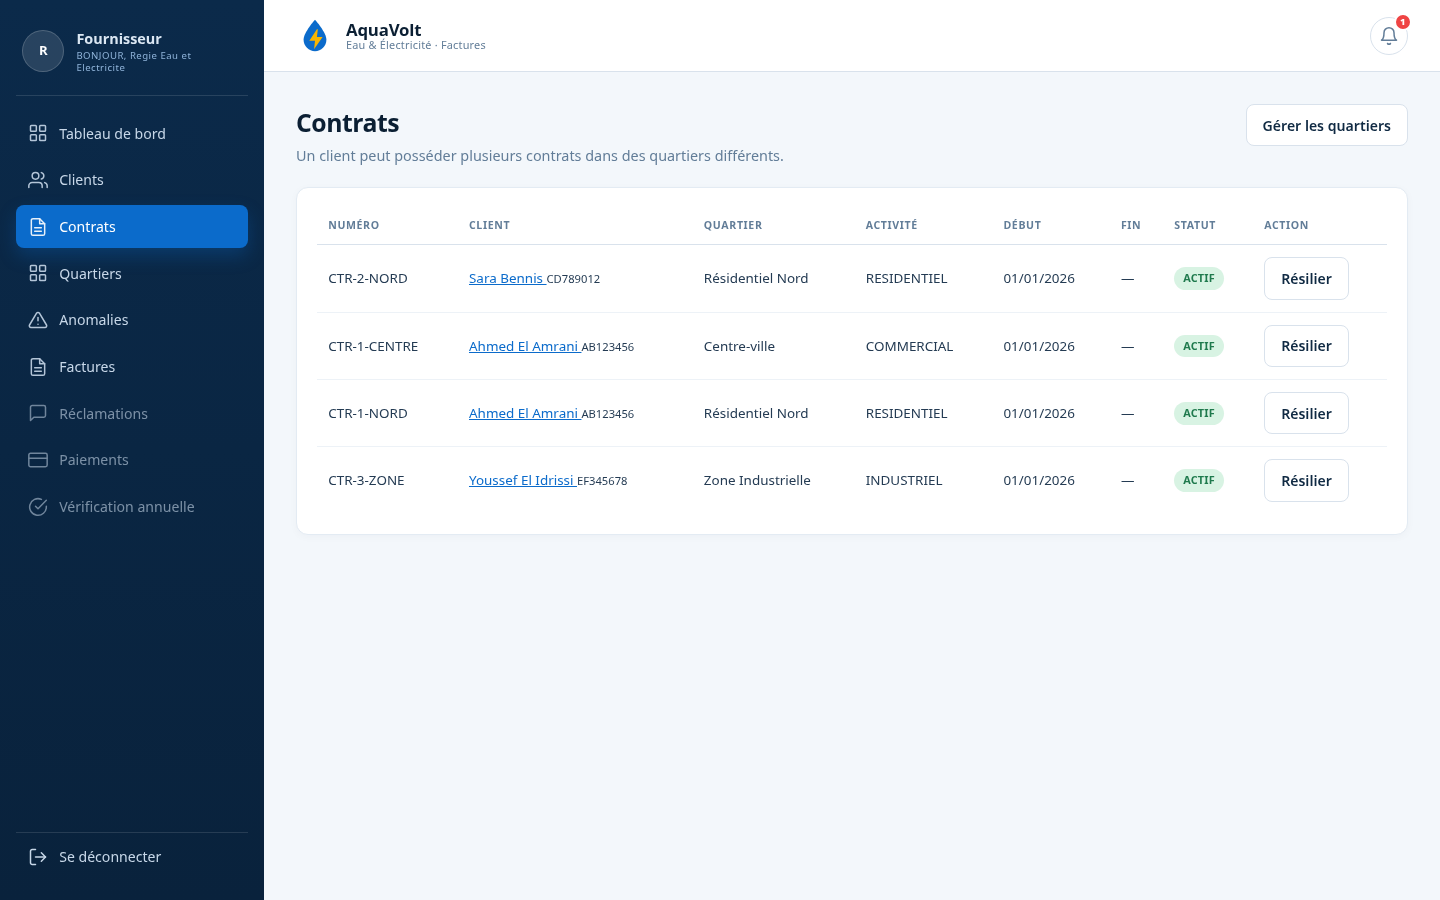
\includegraphics[width=0.92\textwidth]{../tests/screenshots/desktop/01_public_auth/14_contract_list.png}
  \caption{Liste des contrats du fournisseur}
  \label{fig:contrats}
\end{figure}

\begin{figure}[H]
  \centering
  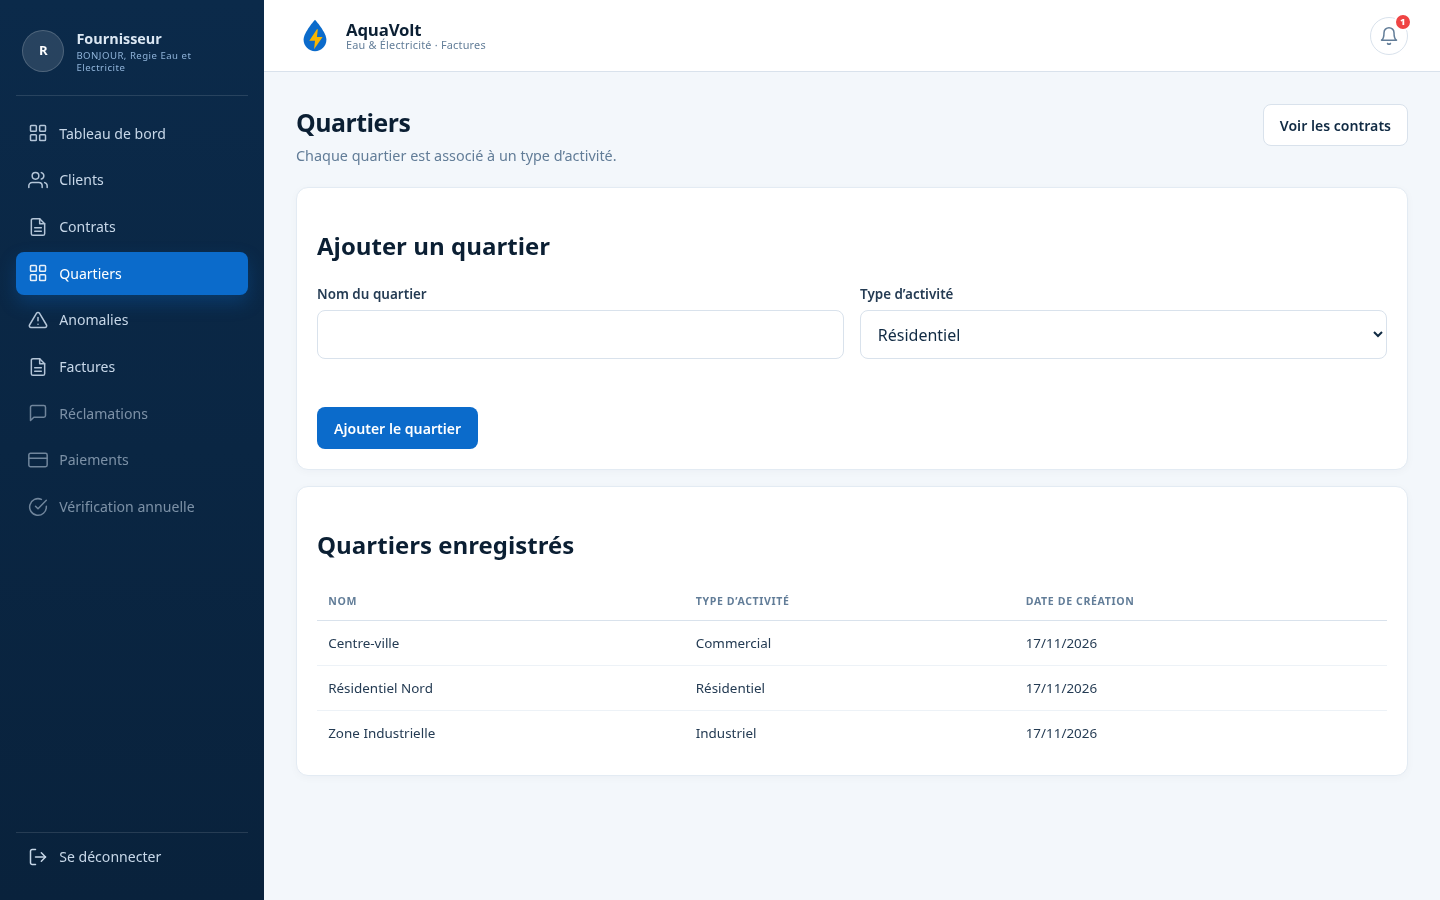
\includegraphics[width=0.92\textwidth]{../tests/screenshots/desktop/01_public_auth/11_quartier_list.png}
  \caption{Gestion des quartiers}
  \label{fig:quartiers}
\end{figure}

\chapter{Saisie des consommations}
\label{chap:consommation}

\todo{décrire la période de saisie, la sélection du contrat, les photos, la validation et le calcul.}

\section{Objectifs}
\section{Période de saisie}
\section{Sélection du contrat}
\section{Formulaire de saisie}
\section{Téléversement des photos}
\section{Validation serveur}
\section{Calcul de la consommation}
\section{Relevé précédent}
\section{Historique et détail}
\section{Tests}

\chapter{Gestion des anomalies}
\label{chap:anomalies}

\todo{décrire les types d'anomalies, la détection, le parcours client, la correction fournisseur et la facturation.}

\section{Objectifs}
\section{Types d'anomalies}
\subsection{Index inférieur}
\subsection{Seuil dépassé}
\section{Détection}
\section{Parcours client}
\section{Correction fournisseur}
\section{Revalidation}
\section{Génération de facture après correction}
\section{Notifications}
\section{Tests}

\chapter{Facturation}
\label{chap:facturation}

\todo{décrire les tranches, la TVA, la génération, le numéro, la transaction et le contenu de la facture.}

\section{Objectifs}
\section{Tarification progressive}
\subsection{Tranches de l'eau}
\subsection{Tranches de l'électricité}
\section{TVA}
\section{Génération de la facture}
\section{Numérotation}
\section{Transaction et unicité}
\section{Contenu de la facture}
\section{Photos des compteurs}
\section{Consultation et contrôle d'accès}
\section{Exemples de calcul}
\section{Tests}

\chapter{Réclamations}
\label{chap:reclamations}

\todo{décrire les types, le dépôt client, le traitement fournisseur, les statuts et les notifications.}

\section{Objectifs}
\section{Types de réclamation}
\subsection{Fuite externe}
\subsection{Fuite interne}
\subsection{Facture}
\subsection{Autre}
\section{Dépôt par le client}
\section{Liste des réclamations}
\section{Traitement par le fournisseur}
\section{Statuts}
\section{Notifications}
\section{Contrôle d'accès}
\section{Tests}

\chapter{Paiements}
\label{chap:paiements}

\todo{décrire les règles, le formulaire fournisseur, le passage à PAYEE, le double paiement et le dashboard.}

\section{Objectifs}
\section{Règles de paiement}
\section{Formulaire fournisseur}
\section{Passage à l'état PAYEE}
\section{Date et référence de paiement}
\section{Double paiement}
\section{Impact sur le tableau de bord}
\section{Notification client}
\section{Tests}

\chapter{Agent et import annuel}
\label{chap:agent}

\todo{décrire le rôle Agent, le fichier annuel, la validation, l'import, les doublons et le rapport.}

\section{Objectifs}
\section{Rôle Agent}
\section{Fichier Consommation\_Annuelle.txt}
\section{Format et validation}
\section{Import automatique}
\section{Gestion des doublons}
\section{Rapport d'import}
\section{Table conso\_annuelle}
\section{Tests}


\chapter{Vérification annuelle}
\label{chap:verification}

\section{Objectifs}

La vérification annuelle permet au fournisseur de comparer les consommations enregistrées mensuellement pour chaque client avec les relevés annuels transmis par l'agent.

Cette opération vise principalement à :
\begin{itemize}
    \item calculer la consommation annuelle à partir des relevés mensuels validés ou facturés ;
    \item comparer les résultats obtenus avec les valeurs du relevé annuel de l'agent ;
    \item identifier les écarts dépassant une tolérance définie ;
    \item permettre au fournisseur de valider ou de rejeter le relevé annuel ;
    \item informer le client de la décision prise.
\end{itemize}

\section{Consommations mensuelles}

La vérification s'appuie sur les enregistrements de la table \texttt{consommation}. Seules les consommations dont le statut est \texttt{VALIDEE} ou \texttt{FACTUREE} sont prises en compte.

Pour chaque client et pour l'année sélectionnée, le système récupère :
\begin{itemize}
    \item les relevés mensuels validés ou facturés ;
    \item les index d'eau et d'électricité ;
    \item les informations permettant de distinguer les différents contrats du client.
\end{itemize}

Le nombre de relevés retenus est également calculé. Le système utilise une constante de douze relevés attendus pour l'année.

\textbf{Remarque :} dans l'implémentation actuelle, ce nombre correspond au nombre d'enregistrements de consommation retenus, et non au nombre de mois distincts. Un client possédant plusieurs contrats peut donc avoir plusieurs relevés pour un même mois.

\section{Relevé annuel de l'Agent}

Les relevés annuels sont enregistrés dans la table \texttt{conso\_annuelle}. Chaque enregistrement contient notamment :
\begin{itemize}
    \item l'identifiant du client ;
    \item l'identifiant de l'agent ayant effectué le relevé ;
    \item la consommation annuelle d'eau ;
    \item la consommation annuelle d'électricité ;
    \item l'année concernée ;
    \item la date de saisie ;
    \item le statut de vérification et la date de décision.
\end{itemize}

La base de données impose une contrainte d'unicité sur le couple \texttt{(id\_client, annee)}. Ainsi, un seul relevé annuel est conservé pour un client et une année.

La page de vérification récupère les relevés annuels disponibles pour les clients du fournisseur connecté. Lorsqu'un relevé existe, ses consommations sont affichées en regard des consommations calculées à partir des relevés mensuels.

\section{Calcul par contrat}

Un même client peut posséder plusieurs contrats. Le calcul annuel doit donc tenir compte de chaque contrat séparément avant d'additionner les résultats.

Pour chaque contrat, le système recherche :
\begin{itemize}
    \item le dernier index validé ou facturé avant l'année sélectionnée ;
    \item le dernier index validé ou facturé pendant l'année sélectionnée.
\end{itemize}

La consommation annuelle d'un contrat est calculée par différence entre ces deux index :

\[
C_{\text{annuelle}} =
\max(0, I_{\text{fin}} - I_{\text{base}})
\]

où :
\begin{itemize}
    \item \(I_{\text{fin}}\) représente le dernier index de l'année ;
    \item \(I_{\text{base}}\) représente le dernier index antérieur à l'année.
\end{itemize}

Si aucun index antérieur n'est disponible, le système utilise zéro comme index de base.

Les consommations calculées pour les différents contrats sont ensuite additionnées afin d'obtenir les consommations annuelles du client :

\[
C_{\text{client}} =
\sum_{i=1}^{n} C_{\text{contrat}_i}
\]

Ce calcul est effectué séparément pour l'eau et l'électricité.

\section{Tolérance}

Le système utilise une tolérance maximale de \(5\,\%\) pour comparer la consommation calculée à partir des relevés mensuels avec celle déclarée par l'agent.

L'écart relatif est calculé à l'aide de la formule suivante :

\[
E(\%) =
\frac{|C_{\text{saisie}} - C_{\text{agent}}|}
{C_{\text{agent}}}
\times 100
\]

où :
\begin{itemize}
    \item \(C_{\text{saisie}}\) désigne la consommation calculée à partir des relevés mensuels ;
    \item \(C_{\text{agent}}\) désigne la consommation annuelle relevée par l'agent.
\end{itemize}

Lorsque la consommation de l'agent est nulle, le système considère l'écart comme égal à \(100\,\%\) si la consommation calculée est positive, et à \(0\,\%\) dans le cas contraire.

Le résultat de l'analyse est déterminé selon les règles suivantes :
\begin{itemize}
    \item \textbf{Sans relevé :} aucun relevé annuel de l'agent n'est disponible ;
    \item \textbf{Incomplet :} le nombre de relevés mensuels enregistrés est inférieur à douze ;
    \item \textbf{Écart :} l'écart calculé pour l'eau ou l'électricité dépasse \(5\,\%\) ;
    \item \textbf{Conforme :} les conditions précédentes ne sont pas réunies.
\end{itemize}

Un écart égal à \(5\,\%\) reste donc dans la tolérance. Le résultat est considéré comme un écart uniquement lorsque la valeur dépasse ce seuil.

\section{Interface fournisseur}

L'interface de vérification est accessible au fournisseur connecté. Elle présente les clients associés à ce fournisseur et les informations nécessaires à la comparaison annuelle.

Un filtre permet de sélectionner l'année à examiner. Par défaut, le système privilégie la dernière année pour laquelle un relevé annuel de l'agent est disponible, ou l'année proposée par la liste lorsque ce relevé n'existe pas.

Pour chaque client, le tableau affiche :
\begin{itemize}
    \item le nom, le prénom et le CIN ;
    \item le nombre de relevés mensuels enregistrés ;
    \item la consommation annuelle d'eau calculée et celle de l'agent ;
    \item l'écart relatif pour l'eau ;
    \item la consommation annuelle d'électricité calculée et celle de l'agent ;
    \item l'écart relatif pour l'électricité ;
    \item le résultat de l'analyse ;
    \item le statut de la décision du fournisseur.
\end{itemize}

Les résultats sont différenciés visuellement à l'aide de badges : conforme, écart à vérifier, saisie incomplète ou relevé agent absent.

\section{Validation et rejet}

Lorsqu'un relevé annuel de l'agent existe, le fournisseur dispose de deux actions :
\begin{itemize}
    \item \textbf{Valider :} enregistrer la décision \texttt{VALIDEE} ;
    \item \textbf{Rejeter :} enregistrer la décision \texttt{REJETEE}.
\end{itemize}

La décision est transmise par une requête POST. Le traitement vérifie le jeton CSRF, le rôle du fournisseur, l'identifiant du client, l'année et la valeur de la décision.

La requête de mise à jour vérifie également que le client appartient bien au fournisseur connecté. Le statut de vérification ainsi que la date de décision sont ensuite enregistrés dans la table \texttt{conso\_annuelle}.

Dans l'implémentation actuelle, la validation ou le rejet reste possible dès lors qu'un relevé annuel existe, même si l'analyse indique un écart ou une saisie incomplète. Le résultat de l'analyse constitue donc une aide à la décision et ne bloque pas automatiquement les actions du fournisseur.

\section{Notification client}

Après l'enregistrement d'une décision, le système tente de créer une notification destinée au client concerné.

Le message dépend de la décision :
\begin{itemize}
    \item après une validation, le client est informé que sa consommation annuelle a été validée ;
    \item après un rejet, le client est informé qu'un écart a été constaté et qu'il doit contacter le fournisseur.
\end{itemize}

La notification est enregistrée avec le type \texttt{VERIFICATION} et contient un lien vers la page des consommations du client.

Si la création de la notification échoue, l'erreur est enregistrée dans le journal technique. Cette situation n'annule pas la décision déjà enregistrée.

\section{Tests}

Les scénarios suivants permettent de vérifier le fonctionnement du module :
\begin{itemize}
    \item vérifier l'affichage des clients associés au fournisseur connecté ;
    \item sélectionner une année et vérifier le chargement des données correspondantes ;
    \item vérifier le calcul annuel d'un client possédant un seul contrat ;
    \item vérifier l'addition des consommations lorsque le client possède plusieurs contrats ;
    \item vérifier le résultat lorsque les douze relevés attendus ne sont pas disponibles ;
    \item vérifier le résultat lorsque l'écart est inférieur, égal ou supérieur à \(5\,\%\) ;
    \item vérifier le cas où aucun relevé annuel de l'agent n'existe ;
    \item vérifier l'enregistrement d'une décision de validation ou de rejet ;
    \item vérifier que le fournisseur ne peut pas décider pour un client appartenant à un autre fournisseur ;
    \item vérifier la création de la notification destinée au client après la décision.
\end{itemize}

Ces scénarios constituent les vérifications fonctionnelles à effectuer sur le module.

\begin{figure}[H]
  \centering
  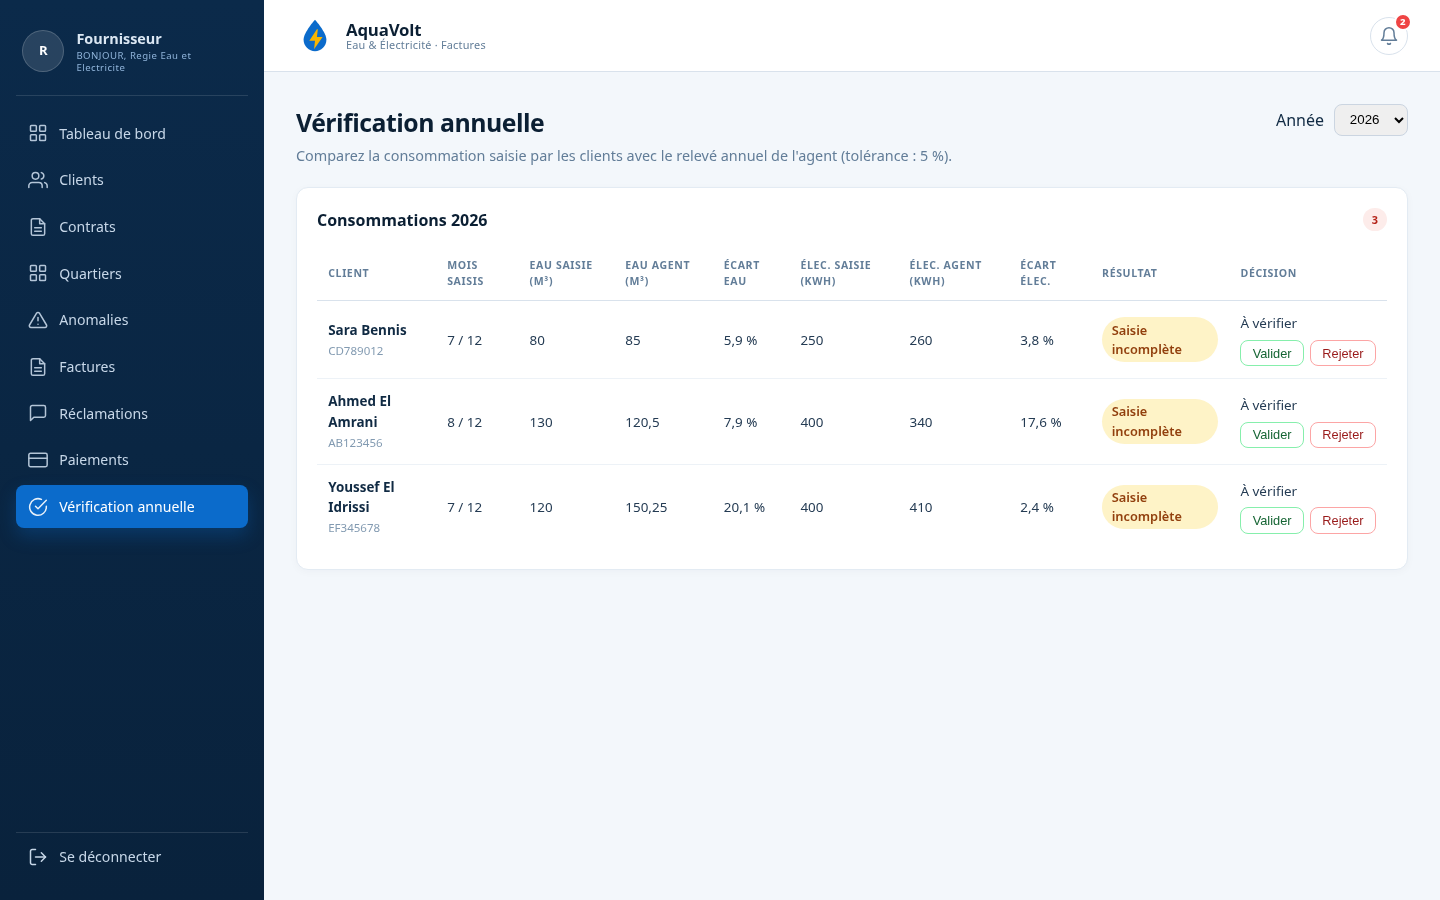
\includegraphics[width=0.95\textwidth]{../tests/final/desktop/10_verification_page.png}
  \caption{Vérification annuelle des consommations}
  \label{fig:verification}
\end{figure}

\chapter{Notifications internes}
\label{chap:notifications}

\todo{décrire la table notification, les événements, la cloche, la page et le marquage comme lu.}

\section{Objectifs}
\section{Table notification}
\section{Événements notifiés}
\section{Cloche et compteur}
\section{Page des notifications}
\section{Marquage comme lu}
\section{Contrôle d'accès}
\section{Tests}


\chapter{Tableau de bord}
\label{chap:dashboard}

\section{Objectifs}

Le tableau de bord constitue un espace de synthèse permettant aux utilisateurs de consulter rapidement les informations essentielles liées à la gestion des consommations et des factures.

Son contenu varie selon le rôle de l'utilisateur connecté. Le fournisseur dispose d'indicateurs financiers et de graphiques permettant de suivre l'activité de ses clients, tandis que le client accède à un résumé de sa propre situation.

\section{Indicateurs fournisseur}

Le tableau de bord du fournisseur présente quatre indicateurs principaux :

\begin{itemize}
    \item \textbf{Total des factures impayées :} montant TTC des factures dont l'état est \texttt{IMPAYEE} pour l'année sélectionnée.
    \item \textbf{Total encaissé :} montant TTC des factures dont l'état est \texttt{PAYEE} pour l'année sélectionnée.
    \item \textbf{Nombre de clients :} nombre de clients rattachés au fournisseur.
    \item \textbf{Anomalies en attente :} nombre d'anomalies dont le statut est \texttt{EN\_ATTENTE}.
\end{itemize}

Ces indicateurs sont calculés à partir des données enregistrées dans la base de données. Les résultats sont affichés sous forme de cartes statistiques afin de faciliter leur consultation.

\section{Total des factures impayées}

Le montant total des factures impayées est calculé en additionnant les montants TTC des factures associées aux clients du fournisseur et dont l'état est \texttt{IMPAYEE}.

Le calcul est réalisé par la méthode \texttt{totaux()} de la classe \texttt{DashboardBD}. Cette méthode utilise une requête SQL avec la fonction d'agrégation \texttt{SUM()} et une condition sur l'état de chaque facture.

Le tableau de bord affiche également le nombre de factures impayées correspondant au montant calculé.

\section{Total encaissé}

Le total encaissé représente la somme des montants TTC des factures dont l'état est \texttt{PAYEE}.

Lorsqu'un fournisseur enregistre le paiement d'une facture, son état est mis à jour dans la base de données. Le tableau de bord prend ensuite en compte ce changement dans le calcul du montant encaissé.

Le nombre de factures payées est également affiché afin de compléter cet indicateur financier.

\section{Évolution mensuelle}

Le tableau de bord permet de suivre l'évolution mensuelle des consommations d'eau et d'électricité facturées pendant l'année sélectionnée.

La méthode \texttt{evolutionMensuelle()} de la classe \texttt{DashboardBD} regroupe les factures par mois à l'aide de la clause SQL \texttt{GROUP BY}. Pour chaque mois, elle calcule :

\begin{itemize}
    \item la somme des consommations d'eau ;
    \item la somme des consommations d'électricité ;
    \item le montant TTC total des factures ;
    \item le nombre de factures correspondantes.
\end{itemize}

La méthode complète ensuite les résultats pour obtenir douze entrées, de janvier à décembre. Lorsqu'aucune facture n'est enregistrée pour un mois, les valeurs correspondantes sont initialisées à zéro.

Cette organisation permet de présenter une évolution annuelle continue, même lorsque certains mois ne comportent aucune facture.

\section{Graphiques}

Les consommations mensuelles sont représentées à l'aide de deux graphiques en barres verticales :

\begin{itemize}
    \item un graphique consacré à la consommation d'eau, exprimée en mètres cubes (m\textsuperscript{3}) ;
    \item un graphique consacré à la consommation d'électricité, exprimée en kilowattheures (kWh).
\end{itemize}

Les graphiques sont générés par la fonction PHP \texttt{chart\_barres()}, définie dans \texttt{config/app.php}. Cette fonction construit directement le code SVG du graphique à partir des données mensuelles fournies.

Chaque graphique représente les douze mois de l'année. La hauteur de chaque barre est proportionnelle à la consommation du mois par rapport à la valeur maximale de l'année. Les noms abrégés des mois sont affichés sous les barres.

Une infobulle SVG permet également d'afficher le nom du mois, la valeur de consommation et son unité lorsque l'utilisateur survole une barre non nulle.

Cette solution utilise le format SVG pour produire les graphiques sans dépendre d'une bibliothèque JavaScript externe.

\section{Filtre par année}

Le fournisseur peut sélectionner une année à partir d'une liste déroulante affichée en haut du tableau de bord.

Les années disponibles sont récupérées par la méthode \texttt{anneesDisponibles()}, qui recherche les années distinctes présentes dans les factures associées aux clients du fournisseur.

Après sélection, le formulaire transmet l'année choisie par une requête HTTP GET. Le contrôleur vérifie que cette année appartient à la liste des années disponibles. Si la valeur demandée n'est pas valide, l'application sélectionne automatiquement l'année la plus récente disponible. En l'absence de factures, l'année courante est utilisée.

Le filtre annuel actualise les montants des factures et les graphiques correspondant à l'année choisie. Le montant total des factures impayées, toutes années confondues, reste également affiché comme information complémentaire.

\section{Tableau de bord client}

Le client dispose d'un tableau de bord simplifié qui présente les informations relatives à son compte.

Trois indicateurs sont affichés :

\begin{itemize}
    \item \textbf{Dernière consommation :} période et statut du dernier relevé enregistré pour le client.
    \item \textbf{Mes factures :} nombre total de factures associées à son compte.
    \item \textbf{Période de saisie :} indique si la période de saisie est ouverte ou fermée.
\end{itemize}

La période de saisie est considérée comme ouverte à partir du 18 du mois. Le tableau de bord affiche également le nombre de jours restants jusqu'à la fin du mois lorsque cette période est ouverte.

Deux raccourcis permettent au client d'accéder directement à la saisie de ses consommations et à la consultation de ses factures.

Concernant les autres rôles, le visiteur non connecté accède à la page d'accueil publique. L'agent est automatiquement redirigé vers son espace d'import annuel.

\section{Tests}

Les scénarios suivants permettent de vérifier le fonctionnement du tableau de bord :

\begin{itemize}
    \item vérifier l'affichage des quatre indicateurs du fournisseur ;
    \item vérifier le calcul des montants impayés et encaissés à partir des états des factures ;
    \item vérifier le nombre de clients et d'anomalies en attente ;
    \item vérifier l'affichage des douze mois dans les graphiques ;
    \item vérifier qu'un mois sans facture présente une valeur nulle ;
    \item vérifier que les graphiques représentent correctement les consommations d'eau et d'électricité ;
    \item sélectionner une autre année et vérifier l'actualisation des indicateurs et des graphiques ;
    \item vérifier le comportement lorsque aucune facture n'est disponible ;
    \item vérifier l'affichage des indicateurs du tableau de bord client ;
    \item vérifier la redirection de l'agent vers son espace d'import annuel.
\end{itemize}

Ces scénarios constituent les vérifications fonctionnelles à effectuer sur le tableau de bord.

\begin{figure}[H]
  \centering
  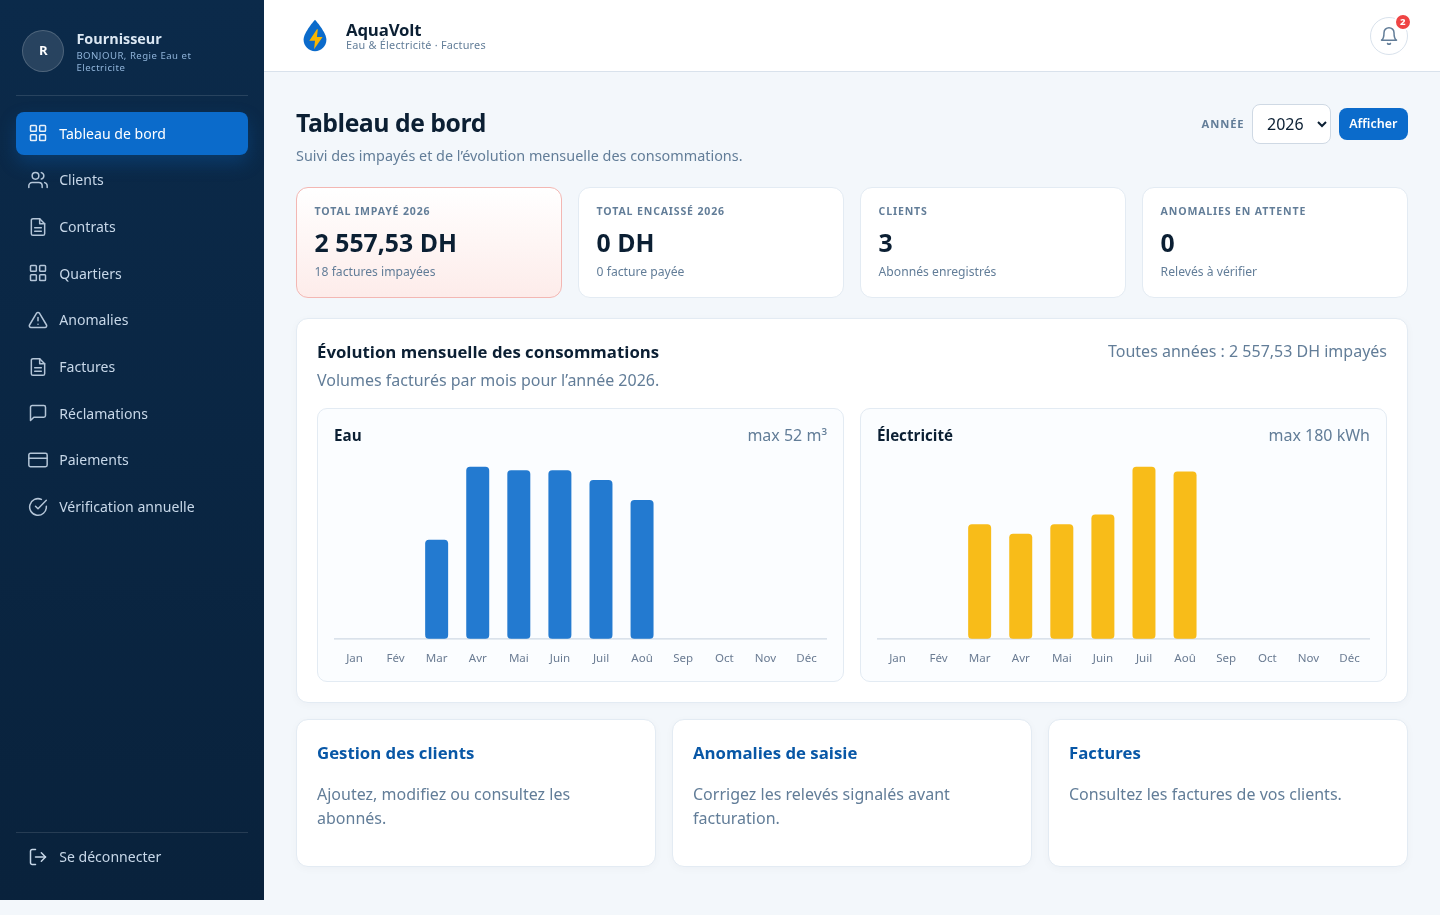
\includegraphics[width=0.95\textwidth]{../tests/final/desktop/06_supplier_dashboard.png}
  \caption{Tableau de bord du fournisseur}
  \label{fig:dashboard}
\end{figure}

\chapter{Tests et validation}
\label{chap:tests}

\todo{présenter la stratégie, les tests fonctionnels, d'intégration, de sécurité, responsive, les captures et les résultats.}

\section{Stratégie de test}
\section{Tests fonctionnels}
\subsection{Authentification}
\subsection{Clients et contrats}
\subsection{Consommation}
\subsection{Anomalies}
\subsection{Factures}
\subsection{Réclamations}
\subsection{Paiements}
\subsection{Agent et import}
\subsection{Vérification annuelle}
\subsection{Notifications}
\section{Tests d'intégration}
\section{Tests de sécurité}
\section{Tests responsive}
\section{Captures d'écran}
\section{Résultats}
\section{Bugs corrigés}
\section{Limites des tests}

\chapter{Bilan, limites et perspectives}
\label{chap:bilan}

\todo{présenter le bilan, les difficultés, les compétences, les limites et les perspectives.}

\section{Bilan fonctionnel}
\section{Difficultés rencontrées}
\section{Compétences acquises}
\section{Limites de la version finale}
\section{Perspectives d'amélioration}

\chapter*{Conclusion générale}
\addcontentsline{toc}{chapter}{Conclusion générale}

Le projet \projectname{} a permis de développer une application web complète de gestion des consommations d'eau et d'électricité et de leurs factures. La version finale couvre la gestion des clients, des quartiers et des contrats, la saisie des consommations, les anomalies, la facturation, les réclamations, les paiements, l'import annuel, la vérification annuelle, les notifications et le tableau de bord.

L'architecture MVC, les transactions, les requêtes préparées et les contrôles d'accès assurent une base maintenable et cohérente. Les tests fonctionnels et responsive ont validé les parcours principaux et les cas d'erreur.

Les perspectives portent sur l'enrichissement du tableau de bord, la pièce jointe des réclamations, la pagination, les notifications e-mail, l'export PDF des factures et l'automatisation des tests.



\chapter*{Glossaire}
\addcontentsline{toc}{chapter}{Glossaire}

\begin{description}[leftmargin=3.2cm,style=nextline]
  \item[Agent] Utilisateur chargé d'importer le fichier annuel des consommations dans l'application.
  
  \item[Contrat] Association entre un client, un quartier et un type d'activité, définissant les conditions de gestion de ses consommations.
  
  \item[CSRF] (Cross-Site Request Forgery) Falsification de requête intersite. Cette attaque consiste à faire exécuter à un utilisateur authentifié une action qu'il n'a pas volontairement demandée. La protection repose notamment sur l'utilisation de jetons CSRF.
  
  \item[Facture] Document généré à partir d'une consommation validée, en appliquant les tarifs correspondants et la TVA.
  
  \item[IHM] Interface homme-machine. Ensemble des éléments permettant à l'utilisateur d'interagir avec l'application.
  
  \item[MVC] (Modèle--Vue--Contrôleur) Architecture logicielle qui sépare la gestion des données, leur présentation et le traitement des actions de l'utilisateur.
  
  \item[PDO] (PHP Data Objects) Extension PHP permettant d'accéder à différentes bases de données à travers une interface commune.
  
  \item[Quartier] Zone géographique associée à un fournisseur et à un type d'activité, utilisée pour organiser les clients et leurs contrats.
  
  \item[Réclamation] Demande formulée par un client concernant un problème lié à son service, notamment une fuite, une facture ou une autre situation.
  
  \item[TVA] Taxe sur la valeur ajoutée. Dans le cadre du projet, son taux est fixé à 18~\%.
  
  \item[XSS] (Cross-Site Scripting) Vulnérabilité permettant d'injecter des scripts malveillants dans une page web consultée par d'autres utilisateurs.
\end{description}
\chapter*{Glossaire}
\addcontentsline{toc}{chapter}{Glossaire}

\begin{description}[leftmargin=3.2cm,style=nextline]
  \item[Agent] Utilisateur chargé de déposer le fichier annuel des consommations.
  \item[Contrat] Rattachement d'un client à un quartier pour une période donnée.
  \item[CSRF] Falsification de requête intersite ; protection par jeton.
  \item[Facture] Document généré après validation d'une consommation.
  \item[IHM] Interface homme-machine.
  \item[MVC] Modèle--Vue--Contrôleur.
  \item[PDO] PHP Data Objects.
  \item[Quartier] Zone géographique associée à un type d'activité.
  \item[Réclamation] Demande client liée à une fuite, une facture ou un autre problème.
  \item[TVA] Taxe sur la valeur ajoutée, fixée à 18~\%.
  \item[XSS] Injection de code HTML ou JavaScript dans une page.
\end{description}


\appendix
\chapter{Routes de l'application}

{\small
\begin{longtable}{>{\raggedright\arraybackslash}p{0.38\textwidth}p{0.12\textwidth}>{\raggedright\arraybackslash}p{0.40\textwidth}}
\caption{Routes principales et contrôleurs associés}\label{tab:routes}\\
\toprule
\textbf{URL} & \textbf{Méthode} & \textbf{Rôle / fonction} \\
\midrule
\endfirsthead
\toprule
\textbf{URL} & \textbf{Méthode} & \textbf{Rôle / fonction} \\
\midrule
\endhead
\texttt{/Auth/login} & GET/POST & Connexion client, fournisseur ou Agent \\
\texttt{/Auth/logout} & GET & Déconnexion \\
\texttt{/Client/all} & GET & Liste et recherche des clients \\
\texttt{/Client/one/\{id\}} & GET & Fiche client et contrats \\
\texttt{/Client/add} & GET/POST & Ajout d'un client \\
\texttt{/Client/update/\{id\}} & GET/POST & Modification d'un client \\
\texttt{/Client/delete/\{id\}} & POST & Suppression conditionnelle \\
\texttt{/Quartier/all} & GET & Liste des quartiers \\
\texttt{/Quartier/add} & POST & Ajout d'un quartier \\
\texttt{/Contrat/all} & GET & Liste des contrats \\
\texttt{/Contrat/add/\{idClient\}} & POST & Ajout d'un contrat \\
\texttt{/Contrat/resilier/\{id\}} & POST & Résiliation d'un contrat \\
\texttt{/Consommation/add} & GET/POST & Saisie d'une consommation \\
\texttt{/Consommation/add/\{id\}} & GET/POST & Correction d'une consommation \\
\texttt{/Consommation/all} & GET & Historique \\
\texttt{/Consommation/one/\{id\}} & GET & Détail \\
\texttt{/Consommation/confirmation/\{id\}} & GET & Confirmation / correction d'anomalie \\
\texttt{/Consommation/confirmer} & POST & Confirmer ou corriger \\
\texttt{/Consommation/facturer} & POST & Génération manuelle d'une facture \\
\texttt{/Facture/all} & GET & Liste des factures \\
\texttt{/Facture/one/\{id\}} & GET & Détail d'une facture \\
\texttt{/Facture/payer/\{id\}} & POST & Paiement fournisseur \\
\texttt{/Anomalie/index} & GET & Liste des anomalies \\
\texttt{/Anomalie/corriger/\{id\}} & GET/POST & Correction fournisseur \\
\texttt{/Reclamation/index} & GET & Liste des réclamations \\
\texttt{/Reclamation/add} & GET/POST & Dépôt d'une réclamation \\
\texttt{/Reclamation/one/\{id\}} & GET & Détail \\
\texttt{/Reclamation/traiter/\{id\}} & POST & Traitement fournisseur \\
\texttt{/Notification/all} & GET & Notifications \\
\texttt{/Notification/lire/\{id\}} & POST & Marquer comme lue \\
\texttt{/Notification/lire\_tout} & POST & Tout marquer comme lu \\
\texttt{/Import/index} & GET/POST & Espace Agent \\
\texttt{/Import/upload} & POST & Import annuel \\
\texttt{/Verification/index} & GET & Vérification annuelle \\
\texttt{/Verification/decider/\{id\}} & POST & Validation / rejet \\
\bottomrule
\end{longtable}
}

\chapter{Schéma SQL}

Le schéma complet de la base de données est fourni ci-dessous.

\begingroup
\lstset{basicstyle=\ttfamily\scriptsize,numbers=none}
\lstinputlisting[language=SQL,caption={Schéma SQL de la base finale}]{../../sql/schema.sql}
\endgroup

\chapter{Exemples de fichiers}

\section{Fichier d'import annuel}

\begin{lstlisting}[caption={Consommation\_Annuelle.txt}]
ID_Client,ID_Agent,ConsommationEau,ConsommationElect,Annee,Date_Saisie
1,1,120.50,340.00,2026,2026-12-15
2,1,85.00,260.00,2026,2026-12-15
3,1,150.25,410.00,2026,2026-12-15
\end{lstlisting}

\section{Fichier d'erreurs}

\begin{lstlisting}[caption={Exemple de lignes invalides}]
ID_Client,ID_Agent,ConsommationEau,ConsommationElect,Annee,Date_Saisie
1,1,130.00,350.00,2026,2026-12-20
99,1,80.00,200.00,2026,2026-12-20
2,1,70.00,180.00
3,1,-5.00,120.00,2026,2026-12-20
\end{lstlisting}

\chapter{Checklist de tests}

\section{Tests fonctionnels}
\begin{itemize}[leftmargin=*]
  \item connexion Agent, client et fournisseur ;
  \item import annuel valide, doublons et fichier d'erreurs ;
  \item dashboard : impayés, encaissé, évolution ;
  \item vérification annuelle et décision ;
  \item dépôt et traitement d'une réclamation ;
  \item paiement total et double paiement ;
  \item gestion des quartiers et contrats ;
  \item saisie de consommation avec deux contrats ;
  \item détection et correction d'anomalies ;
  \item génération et consultation des factures ;
  \item notifications et marquage comme lu.
\end{itemize}

\section{Tests de sécurité}
\begin{itemize}[leftmargin=*]
  \item accès selon le rôle ;
  \item CSRF ;
  \item échappement HTML ;
  \item requêtes préparées ;
  \item contrôle des uploads ;
  \item accès à une facture d'un autre client.
\end{itemize}

\section{Tests responsive}
\begin{itemize}[leftmargin=*]
  \item desktop 1440~px ;
  \item tablette 1024~px ;
  \item mobile 390~px ;
  \item tableaux scrollables ;
  \item navigation mobile.
\end{itemize}

\chapter{Captures complémentaires}

\section{Vue desktop}

\begin{figure}[H]
  \centering
  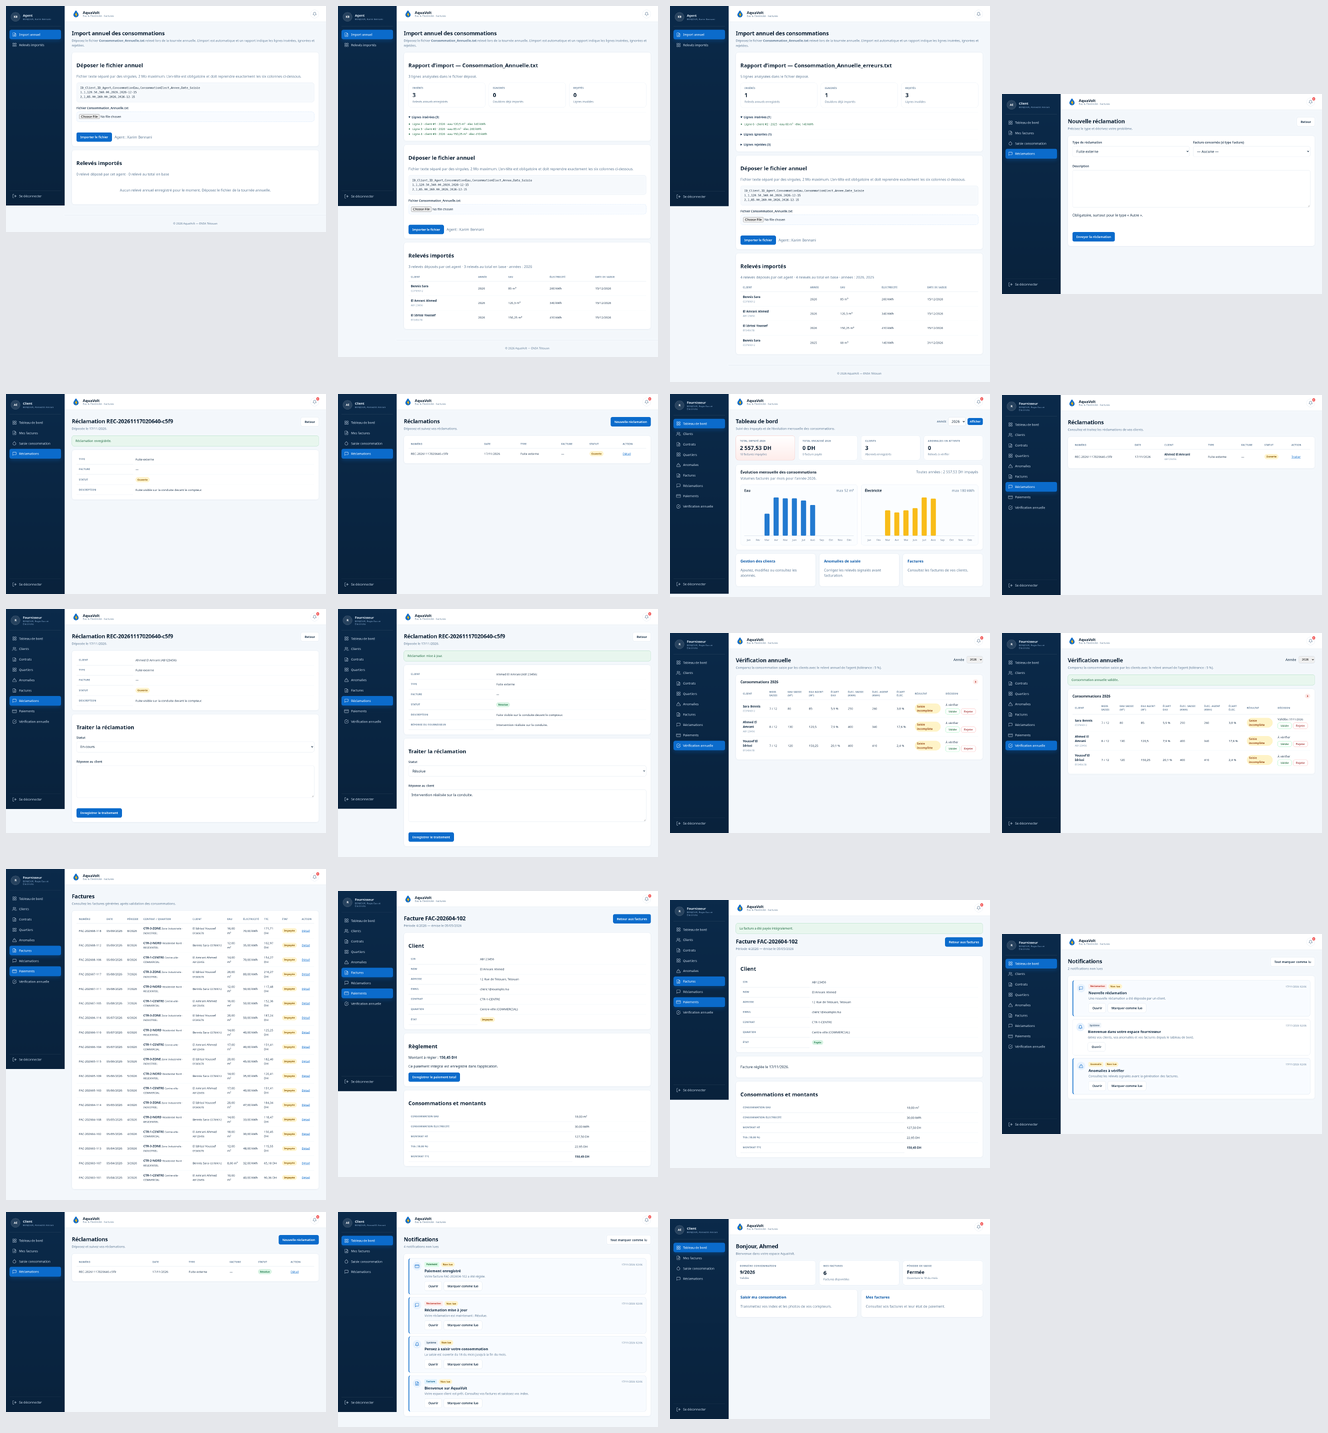
\includegraphics[width=\textwidth]{../tests/final/final_contact_desktop.png}
  \caption{Planche contact des tests desktop}
  \label{fig:contact-desktop}
\end{figure}

\section{Vue responsive}

\begin{figure}[H]
  \centering
  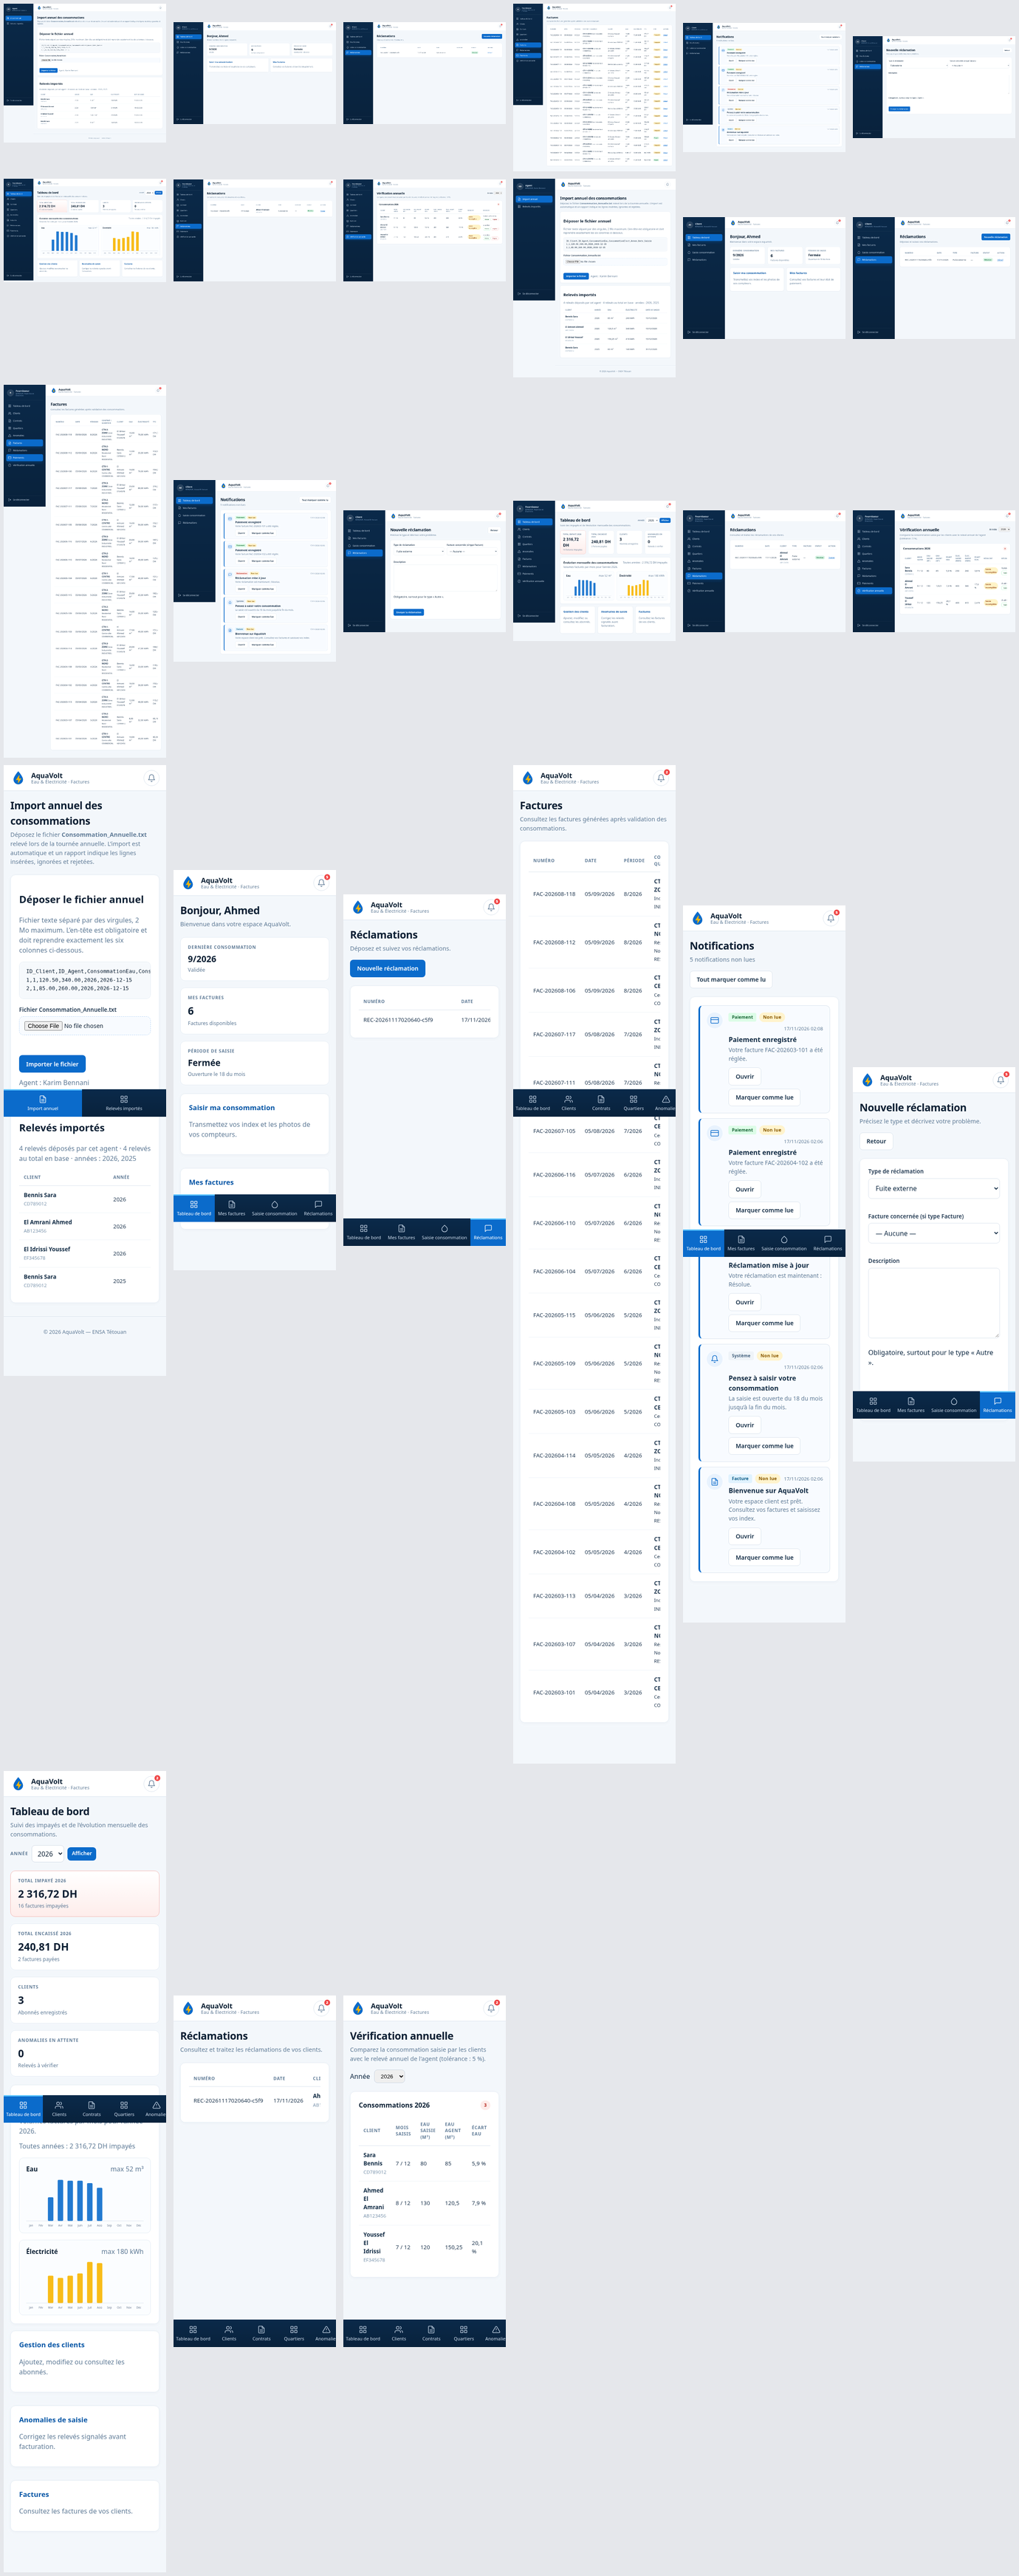
\includegraphics[width=\textwidth]{../tests/final/final_contact_responsive.png}
  \caption{Planche contact desktop, tablette et mobile}
  \label{fig:contact-responsive}
\end{figure}

\chapter{Organisation Git et livraison}

\section{Branches principales}
\begin{itemize}[leftmargin=*]
  \item \texttt{main} : branche stable ;
  \item \texttt{integration/final} : intégration des modules ;
  \item branches de fonctionnalités : clients, consommation, factures, notifications, quartiers, réclamations, Agent.
\end{itemize}

\section{Pull Requests}
\begin{itemize}[leftmargin=*]
  \item PR \#1 : version Alpha fonctionnelle ;
  \item PR \#2 : corrections UI/UX ;
  \item PR \#3 : rapport Alpha ;
  \item PR \#5 : quartiers et contrats ;
  \item PR \#6 : notifications ;
  \item PR \#7 : anomalies ;
  \item PR \#8 : tests manuels ;
  \item PR \#9 : intégration finale.
\end{itemize}

\section{Version livrée}
\begin{itemize}[leftmargin=*]
  \item version : \texttt{v1.0-final} ;
  \item date : \today ;
  \item dépôt : \url{https://github.com/AbdellahBouarguan/miniprojectI_WEB}.
\end{itemize}


\end{document}
